% !TeX spellcheck = en_US
\documentclass[english,twoside]{article}
\usepackage[T1]{fontenc}
\usepackage[utf8]{inputenc}
\usepackage{lmodern}
\usepackage[a4paper]{geometry}
\usepackage{babel}
\usepackage{graphicx}
\usepackage{float}
\usepackage{hyperref}
\usepackage{listings}
\usepackage{color}
\usepackage{siunitx}
\usepackage{csquotes}
\usepackage[printonlyused,footnote]{acronym}
\usepackage{pdflscape}
\usepackage{subcaption}
\usepackage{pdfpages}
\usepackage{afterpage}
\usepackage{wrapfig}
\usepackage{fancyhdr}
\usepackage{amsmath}
\usepackage[export]{adjustbox}
\fancyhead{}
\fancyhead[RO,LE]{Full-Wave Design of Coaxial to Waveguide Transitions and Waveguide Mode Transducers}
\fancyfoot{}
\fancyfoot[LE,RO]{\thepage}
\fancyfoot[LO,RE]{\rightmark}
%\fancyfoot[CO,RE]{Miguel González}
\pagestyle{fancy}
\hyphenation{wa-ve-gui-de}
%\usepackage{appendix}

\newcommand\pro{\item[$+$]}
\newcommand\con{\item[$-$]}

\input{"/Users/miguel/Google Drive/Aficiones/listings.tex"}

\newcommand\tab[1][1cm]{\hspace*{#1}}
\providecommand{\keywords}[1]
{
  {\small	
  \textbf{\textit{Keywords---}} #1}
}

\providecommand{\keywordsde}[1]
{
  {\small	
  \textbf{\textit{Schlüsselworte---}} #1}
}

\title{Full-Wave Design of Coaxial to Waveguide Transitions and Waveguide Mode Transducers}
\author{Miguel González Calvo}
\begin{document}
%	\afterpage{\null\newpage}
	\includepdf[pages=-]{pdf/cover.pdf}
	\newpage
	
	\thispagestyle{empty}
	\Large \textbf{Master's Thesis}
	\normalsize
	
	\vspace{20pt}
	
	\begin{tabular}{ll}
		\textbf{Title} & Full-Wave Design of Coaxial to Waveguide Transitions and\\ & Waveguide Mode Transducers. \\[2ex]
		\textbf{Author}  & Miguel González Calvo. \\[2ex]
		\textbf{Tutor} & José Ramón Montejo Garai. \\[2ex]
		\textbf{Department}	& Señales, Sistemas y Radiocomunicaciones.
	\end{tabular}

	\vspace{40pt}
	\Large \textbf{Composition of the Tribunal}
	\normalsize
	\vspace{20pt}
	
	\begin{tabular}{ll}
		\textbf{President} & \\[2ex]
		\textbf{Vocal} & \\[2ex]
		\textbf{Secretary} & \\[2ex]
		\textbf{Substitute} & 
	\end{tabular}
	
	\vspace{40pt}
	The members of the aforementioned tribunal agree on giving the grade of: \\
	
	\vspace{40pt}
	\hfill Madrid, \_\_ of January of 2019
	
	
%	\vspace{\stretch{1}}
	
	
	
	\includepdf[pages=-]{pdf/cover_internal.pdf}
	
	\thispagestyle{empty} 
	\clearpage \mbox{} \clearpage
	
	\pagenumbering{roman}
	\section*{Summary}
		The purpose of this work was to provide an approach to design, simulate, optimize and analyze several coaxial to waveguide transitions with different output modes and waveguide mode transducers (both rectangular and circular types). Both transitions and mode transducers are devices of the utmost importance and widely used in the radio-frequency field, and nowadays the existence of CAD and computational electromagnetics techniques allows for very efficient design procedures dealing with unprecedentedly demanding specifications, leaving behind the traditional heuristic and laboratory adjustment methods. First, a traditional \ac{TEM} coaxial mode to \ac{TE}\textsubscript{10} rectangular waveguide mode transition was designed by making use of a metallic protuberance to improve the matching properties without the need of any tuning screw providing a very good electric response with a simple geometry throughout the complete \ac{WR}75 usable band. Secondly, two designs for a non-conventional \ac{TEM} coaxial mode to \ac{TE}\textsubscript{20} rectangular waveguide mode transition were developed by achieving the electrical geometry of the output mode with two different feeding configurations; the usage of tuning screws and an appropriate feeding structure allowed for a response with a $\SI{3.43}{\percent}$ of band. After the coaxial to waveguide transitions, the design of several waveguide mode transducers was conducted: a \ac{TE}\textsubscript{10} rectangular waveguide mode to \ac{TM}\textsubscript{01} circular waveguide mode transducer was designed by using a proposal and a second one by exploring new geometries with an own design achieving a $\SI{15.38}{\percent}$ of band with a central frequency $f_0\approx\SI{13.25}{\giga\hertz}$; an easily manufacturable \ac{TE}\textsubscript{10} rectangular waveguide mode to \ac{TE}\textsubscript{20} rectangular waveguide mode transducer with a symmetric iris to achieve the latter mode field configuration; a narrow-band \ac{TE}\textsubscript{20} rectangular waveguide mode to TE\textsubscript{01} circular waveguide mode transducer by the design of intermediate sections to adapt progressively the field configuration to the one of the desired mode (flared-type); and a TE\textsubscript{10} rectangular waveguide mode to TE\textsubscript{01} circular waveguide mode transducer based on the Marié-type mode converter with an outstanding usable bandwidth (the complete Q-band, $\SI{41}{\percent}$ of band) for a return loss over $\SI{20}{\decibel}$. Finally, two prototypes of the latter device were manufactured via Additive Manufacturing (\ac{SLS}) and measured in back-to-back configuration to further validate the obtained theoretical results; not only did these measurements validate the simulated results by showing a high degree of correlation between the measured and simulated values but also proved the suitability of this manufacturing technique for this sort of flared-type structures, providing in this measurements a worst measured value of conversion efficiency of $\SI{83}{\percent}$ in the whole Q-band, an excellent result which reveals the fact that even at such high frequencies, where traditionally only machining manufacturing processes were used, Additive Manufacturing has an extraordinary potential.\\

	
	\keywords{waveguide transition, waveguide mode transducer, mode-conversion purity, additive manufacturing, selective laser sintering}\\

	\newpage
	\section*{Zusammenfassung}
		
		Der Zweck dieser Arbeit war, einen Ansatz aufzuzeigen, verschiedene Übergänge von Koaxialkabel auf Hohlleiter mit variierenden Output-Moden und verschiedene Wandler für Hohlleitermoden (sowohl rechteckige als auch kreisförmige Varianten) zu entwerfen, zu simulieren, zu optimieren und zu analysieren. Hohlleiterübergänge und -wandler sind Geräte von höchster Wichtigkeit und finden breite Anwendung im Bereich der Hochfrequenztechnik. Heutzutage ermöglichen die Existenz von CAD und computerunterstützter Elektromagnetik ausgesprochen effiziente Designprozeduren, die Spezifikationen von niedagewesener Komplexität bedienen können und somit traditionelle, heuristische und laboratorische Anpassungsmethoden ablösen. Zuerst wurde ein traditioneller \ac{TEM} Koaxialkabelmode zu \ac{TE}\textsubscript{10} Rechteckighohlleitermode Übergang entworfen, indem eine metallische Protuberanz genutzt wurde, um den Reflexionsfaktor zu verbessern, ohne eine Stellschraube zu benötigen, was mithilfe einer simplen Geometrie zu einer sehr guten elektrischen Reaktion über das gesamte nutzbare \ac{WR}75 Frequenzband führt. Danach wurden zwei Entwürfe für nichtkonventioneller  \ac{TEM} Koaxialkabelmode zu \ac{TE}\textsubscript{20} Rechteckighohlleitermode Übergang entwickelt, indem die elektrische Geometrie der Output-Mode mit zwei verschiedenen Einspeisekonfigurationen erreicht wurde. Hierbei ermöglichte die Nutzung von Einstellschrauben und einer adäquaten Einspeisevorrichtung eine $\SI{3.43}{\percent}$-ige Bandbreite. Nach den Koaxialkabel auf Hohlleiterübergängen wurden mehrere Wandler für Hohlleitermoden entworfen: ein \ac{TE}\textsubscript{10} Rechteckighohlleitermode zu \ac{TM}\textsubscript{01} kreisförmigen Hohlleitermode Wandler wurde auf der Grundlage eines  Designvorschlags, ein weiterer auf Basis eines eigenen Designs entworfen, welcher eine $\SI{15.38}{\percent}$-ige Bandbreite mit $f_0\approx\SI{13.25}{\giga\hertz}$ erzielte; ein einfach zu produzierender  \ac{TE}\textsubscript{10} Rechteckighohlleitermode zu  \ac{TE}\textsubscript{20} Rechteckighohlleitermode Wandler mit einer symmetrischen Iris, um die letztere Feldkonfiguration zu erreichen; ein Schmalband-\ac{TE}\textsubscript{20} Rechteckighohlleitermode zu TE\textsubscript{01} kreisförmigen Hohlleitermode Wandler indem Zwischensektionen entworfen wurden, um die Feldkonfiguration schrittweise an die des gewünschten Modes anzupassen (flared-type); ein \ac{TE}\textsubscript{10} Rechteckighohlleitermode zu \ac{TE}\textsubscript{01} kreisförmigen Hohlleitermode Wandler basierend auf dem Marié-type Modewandler mit einer herausragenden nutzbaren Bandbreite (das komplette Q-Band, $\SI{41}{\percent}$-ige Bandbreite) für eine Reflexionsdämpfung von über $\SI{20}{\decibel}$. Zuletzt wurden zwei Prototypen des letzten Geräts mithilfe von Additive Manufacturing (\ac{SLS}) hergestellt und in einer back-to-back Konfiguration gemessen, um die zuvor theoretisch erhaltenen Ergebnisse zu validieren. Die Korrelation zwischen den gemessenen und simulierten Werten, welche die Messungen der Prototypen zeigten, validierten nicht nur die simulierten Messergebnisse, sondern zeigten auch die Tauglichkeit dieses Herstellungsprozesses für diese Art von flared-type Geräten. Über das gesamte Q-Band zeigten die Messergebnisse eine Modenumwandlungseffizienz von mindestens $\SI{83}{\percent}$ - ein herausragendes Ergebnis, welches beweist, dass selbst bei so hohen Frequenzen, bei denen traditionell nur Fräsungen eingesetzt wurden, Additive Manufacturing ein außergewöhnliches Potenzial zeigt.\\
		
	\keywordsde{Hohlleiterübergang, Hohlleiterwandler, Reinheit der Modenumwandlung, Additive Manufacturing, Selective Laser Sintering}
		
	\newpage
	
	\tableofcontents
	\newpage
	\listoffigures
	\listoftables


	\newpage
	\section*{Acronyms}
	
	\begin{acronym}
		\acro{WR}{Waveguide Rectangular (EIA)}
		\acro{WC}{Waveguide Circular}
		\acro{TE}{Transversal Electric}
		\acro{TM}{Transversal Magnetic}
		\acro{TEM}{Transversal Electro-Magnetic}
		\acro{SMA}{SubMiniature version A}
		\acro{EIA}{Electronic Industries Alliance}
	    \acro{PEC}{Perfect Electric Conductor}
	    \acro{AM}{Additive Manufacturing}
	    \acro{SLS}{Selective Laser Sintering}
	    \acro{VNA}{Vector Network Analyzer}
	    \acro{MW}{Magnetic Wall}
	    \acro{EW}{Electric Wall}
   	\end{acronym}

	\newpage \pagenumbering{arabic}
	
	\section{Introduction}
		Although waveguides' ordinary operation mode is the usage of only one propagating mode corresponding to the one with lowest cut-off frequency, there are some special applications in which the usage of a higher order mode is of the utmost importance for several reasons. As described in the theory \cite{collin}, mode decomposition provides with a description of both electric and magnetic fields via an infinite summation of eigenvalues with eigenfunctions, which each can be treated independently. This fact was mathematically proven by Lord Rayleigh in 1897 for circular and rectangular cross sections as the existence of a cut-off frequency, defined as the frequency below which all lower frequencies are attenuated by the waveguide and above which all higher frequencies propagate within the waveguide. Nowadays the usage of waveguides is limited by other technologies for RF transmission such as coaxial cables, microstrip lines, striplines, slotlines or coplanar waveguides which can be compact, cheaper and provide high integration capabilities. However, although more expensive and bulkier, waveguides are still in use due to the high power handling capability and low loss.\\
		
		Manufacturing, thus, is sophisticated and waveguide materials such as copper and silver are relatively expensive. Plus, one can take advantage of employing a higher order mode as main transmission mode instead of the fundamental mode in order to reduce the losses for high power applications among other advantages.\\
		
		For most of these applications with higher modes as main transmission modes it is necessary a transducer which takes at the input the fundamental mode of the transmission media and outputs to a transmission media with another mode as main transmitting mode. These devices which such functionality are referred to as mode transducers.\\
		
		In the present document, an approach to the design and simulation of waveguide mode transducers and coaxial to waveguide transitions is presented by using the software \texttt{CST Studio} with different solvers, providing with a full-wave solution of the designs of interest. Scattering parameters are chosen as the figure of merit for comparison and optimization, providing an overview of how efficient the transducer is for a certain frequency, mode and combination of input-output.\\
		
		The designs carried out in this work are the following:		
		\begin{enumerate}
			\item Transitions:
			\begin{itemize}
				\item \ac{TEM} coaxial mode to \ac{TE}\textsubscript{10} rectangular waveguide mode.
				\item \ac{TEM} coaxial mode to \ac{TE}\textsubscript{20} rectangular waveguide mode (two different geometries).
			\end{itemize}
			\item Mode Transducers:
			\begin{itemize}
				\item \ac{TE}\textsubscript{10} rectangular waveguide mode to \ac{TM}\textsubscript{01} circular waveguide mode (two different geometries).
				\item \ac{TE}\textsubscript{10} rectangular waveguide mode to \ac{TE}\textsubscript{20} rectangular waveguide mode.
				\item \ac{TE}\textsubscript{20} rectangular waveguide mode to \ac{TE}\textsubscript{01} circular waveguide mode. 
				\item \ac{TE}\textsubscript{10} rectangular waveguide mode to \ac{TE}\textsubscript{01} circular waveguide mode.
			\end{itemize}
		\end{enumerate}
		
		A progressive approach through different mode transducers is made with the ultimate goal of the complete design and verification process: design, simulation, optimization, manufacturing and measuring of a Marié-type \ac{TE}\textsubscript{01} circular waveguide mode transducer. The aforementioned process includes the manufacturing done by the additive manufacturing technique and the measurement by using the back-to-back technique allowing a suitable measurement of the insertion loss of the connection of two similar devices and besides, a good estimation of the return loss level. In order to verify the irrelevant influence of the other propagating modes four different connection angles, 0, 45, 90 and 180 degrees between the two devices will be arranged in the measurements.
	
  

	\newpage
	\section{General Considerations}
		Dimensions of the rectangular waveguide are subject to the definition provided by the \ac{EIA} as shown in Table \ref{table:wr_dimensions}. Theoretical single mode usable band is determined by both cut-off frequencies: lowest order mode and next mode (Tables \ref{table:wr22_modes} and \ref{table:wr75_modes}).\\
		
		Dimensions of the \ac{SMA} connector are set to $D_{\mathrm{in}}=\SI{1.27}{\milli\metre}$ and $D_{\mathrm{out}}=\SI{4.115}{\milli\meter}$ for all the designs with this connector.\\
			
		Conversion efficiency is determined by the following equation:
		
		\begin{equation} \label{eq:conversion_eff}
			\mathrm{CE [\%] = 100 \cdot |s_{21}|^2}
		\end{equation}
		%
		where $s_{21}$ is the transmission scattering parameter for the desired mode.\\
    
    In order to provide with a figure of merit for each transition, the bandwidth for which the efficiency is under a certain threshold is chosen. Given that for each transition the number of modes is different and not only the return loss is the key driver but also higher order modes presence, this bandwidth is defined as the frequencies for which the design is providing an efficiency above $\SI{99}{\percent}$, corresponding to a return loss higher than $\SI{20}{\decibel}$.\\
    
    Please note that unless otherwise stated, the mentioned simulation results are obtaining by simulating a lossless conductor, i.e. metallic component simulated as \ac{PEC} (infinite conductivity, $\sigma \to \infty$), and using lossless Teflon ($\varepsilon=2.1$) as main dielectric material.\\
    
    In the following pages, mode electric and magnetic symmetries are taken into account. Please note that in the tables they are referred to by \ac{MW} and \ac{EW}.
    
    \subsection{Rectangular waveguides considerations}
      Cut-off frequencies for a rectangular waveguide are obtained with the following equation \cite{collin}:
	  
	  \begin{equation} \label{eq:wr_fc}
	  	f_c=\frac{1}{2\pi\sqrt{\mu\epsilon}}\sqrt{\left(\frac{m\pi}{a}\right)^2+\left(\frac{n\pi}{b}\right)^2}
	  \end{equation}	
      %
      where:
      
      \begin{itemize}
        \item $\mu$ is the electromagnetic permeability of the material inside the waveguide.
        \item $\epsilon$ is the electromagnetic permittivity of the material inside the waveguide.
        \item $a$ is the horizontal dimension of the waveguide.
        \item $b$ is the vertical dimension of the waveguide.
        \item $m$ is the number of variations of the electric field in the x-axis.
        \item $n$ is the number of variations of the electric field in the y-axis.
      \end{itemize}
  
  	Attenuation due to conductor loss is given in \cite{pozar}:
  	\begin{equation}
  		\alpha_{c,\textrm{TE}_\textrm{10}} = \frac{R_s}{\eta b}\frac{\left[1+\frac{2b}{a}\left(\frac{f_c}{f}\right)^2\right]}{\sqrt{1-\left(\frac{f_c}{f}\right)^2}}
  	\end{equation}
    %
    where the conductor surface resistivity is $R_s=\sqrt{\frac{\omega\mu}{2\sigma}}$ and $\eta=\sqrt{\frac{\mu}{\varepsilon}}$.\\
    
      \noindent The equations for the rectangular waveguide \ac{TE} modes are:
      
      \begin{subequations}
      	\begin{equation}
      		E_x=A_{\textrm{mn}} \frac{n\pi}{b\varepsilon} \cos\left(\frac{m\pi}{a}x\right) \sin\left(\frac{n\pi}{b}y\right) e^{-j\beta_z z}
      	\end{equation}
      	\begin{equation}
      		E_y=-A_{\textrm{mn}} \frac{m\pi}{a\varepsilon} \sin\left(\frac{m\pi}{a}x\right) \cos\left(\frac{n\pi}{b}y\right) e^{-j\beta_z z}
      	\end{equation}
      	\begin{equation}
      		E_z=0
      	\end{equation}
      	\begin{equation}
      		H_x=   A_{\textrm{mn}} \frac{m\pi\beta_z}{a\omega\mu\varepsilon} \sin\left(\frac{m\pi}{a}x\right) \cos\left(\frac{n\pi}{b}y\right) e^{-j\beta_z z}
      	\end{equation}
      	\begin{equation}
      		H_y=   A_{\textrm{mn}} \frac{n\pi\beta_z}{b\omega\mu\varepsilon} \cos\left(\frac{m\pi}{a}x\right) \sin\left(\frac{n\pi}{b}y\right) e^{-j\beta_z z}
      	\end{equation}
      	\begin{equation}
      		H_z=-j A_{\textrm{mn}} \frac{\beta_c^2}{\omega\mu\varepsilon}    \cos\left(\frac{m\pi}{a}x\right) \cos\left(\frac{n\pi}{b}y\right) e^{-j\beta_z z}
      	\end{equation}      	
      \end{subequations}
      %
      where:
      \begin{itemize}
        \item $m=0,1,2,...$
        \item $n=0,1,2,...$
        \item $m=n\neq 0$
        \item $A_{\textrm{mn}}$ is an arbitrary amplitude constant composed of the remaining constants $A$ and $C$ from the general solution for $h_z(x,y)=(A\cos k_x x + B\sin k_x x)(C\cos k_y y +D\sin k_y y)$, where $H_z(x,y,z)=h_z(x,y) e^{-j\beta_z z}$. Eq. 3.73 \cite{pozar}.
        \item $\beta_z(f\geq f_c)=\beta \sqrt{1-\left(\frac{f_c}{f}\right)^2}$
        \item $\beta_c=\sqrt{\left(\frac{m\pi}{a}\right)^2+\left(\frac{n\pi}{b}\right)^2}$
        \item $\beta = \frac{2\pi}{\lambda}=\omega\sqrt{\mu\varepsilon}$
      \end{itemize}
      
      \noindent The equations for the rectangular waveguide \ac{TM} modes are:
      
      \begin{subequations}
      	\begin{equation}
      		E_x=   B_{\textrm{mn}} \frac{m\pi\beta_z}{a\omega\mu\varepsilon} \cos\left(\frac{m\pi}{a}x\right) \sin\left(\frac{n\pi}{b}y\right) e^{-j\beta_z z}
      	\end{equation}
      	\begin{equation}
      		E_y=-  B_{\textrm{mn}} \frac{n\pi\beta_z}{b\omega\mu\varepsilon} \sin\left(\frac{m\pi}{a}x\right) \cos\left(\frac{n\pi}{b}y\right) e^{-j\beta_z z}
      	\end{equation}
      	\begin{equation}
      		E_z=-j B_{\textrm{mn}} \frac{\beta_c^2}{\omega\mu\varepsilon}    \sin\left(\frac{m\pi}{a}x\right) \cos\left(\frac{n\pi}{b}y\right) e^{-j\beta_z z}
      	\end{equation}
      	\begin{equation}
      		H_x= B_{\textrm{\textrm{mn}}} \frac{n\pi}{b\mu} \sin\left(\frac{m\pi}{a}x\right) \cos\left(\frac{n\pi}{b}y\right) e^{-j\beta_z z}
      	\end{equation}
      	\begin{equation}
      		H_y=-B_{\textrm{\textrm{mn}}} \frac{m\pi}{a\mu} \cos\left(\frac{m\pi}{a}x\right) \sin\left(\frac{n\pi}{b}y\right) e^{-j\beta_z z}
      	\end{equation}
      	\begin{equation}
      		H_z=0
      	\end{equation}      	
      \end{subequations}
      %
      where:
      \begin{itemize}
        \item $m=1,2,3,...$
        \item $n=1,2,3,...$
        \item $B_{\textrm{\textrm{mn}}}$ is an arbitrary amplitude constant composed of the remaining constants $B$ and $D$ from the general solution for $e_z(x,y)=(A\cos k_x x + B\sin k_x x)(C\cos k_y y +D\sin k_y y)$, where $E_z(x,y,z)=e_z(x,y) e^{-j\beta_z z}$. Eq. 3.97 \cite{pozar}.
        \item $\beta_z(f\geq f_c)=\beta \sqrt{1-\left(\frac{f_c}{f}\right)^2}$
        \item $\beta_c=\sqrt{\left(\frac{m\pi}{a}\right)^2+\left(\frac{n\pi}{b}\right)^2}$
        \item $\beta = \frac{2\pi}{\lambda}=\omega\sqrt{\mu\varepsilon}$
      \end{itemize}
      
      \begin{table}[H]
        \centering
        \caption{Used WR dimensions.}
        \begin{tabular}{c|c|c|c}
          \ac{EIA} name & Recommended frequency &  $a$  & $b$ \\
          \hline
          WR75 & 10-$\SI{15}{\giga\hertz}$ &  $\SI{0.75}{in}$ ($\SI{19.05}{\milli\metre}$) & $\SI{0.375}{in}$ ($\SI{9.525}{\milli\metre})$\\
          WR22 & 33-$\SI{50}{\giga\hertz}$ &  $\SI{0.224}{in}$ ($\SI{5.6896}{\milli\metre}$) & $\SI{0.112}{in}$ ($\SI{2.8448}{\milli\metre})$
        \end{tabular}
        \label{table:wr_dimensions}
      \end{table}
      
      \begin{table}[H]
        \centering
        \caption{Mode list for WR75 without symmetry constraints.}
        \begin{tabular}{c|c|c|c|c}
          Mode no. & Mode name & Cut-off frequency [GHz] & xz-symmetry & yz-symmetry\\
          \hline
          1 & TE\textsubscript{10} & $\num{7.8686}$ & EW & MW\\
          2 & TE\textsubscript{20} & $\num{15.737}$ & EW & EW\\
          3 & TE\textsubscript{01} & $\num{15.737}$ & MW & EW\\
          4 & TE\textsubscript{11} & $\num{17.595}$ & MW & MW\\
          5 & TM\textsubscript{11} & $\num{15.595}$ & MW & MW\\
          6 & TE\textsubscript{21} & $\num{22.256}$ & MW & EW\\
          7 & TM\textsubscript{21} & $\num{22.256}$ & MW & EW\\
          8 & TE\textsubscript{30} & $\num{23.606}$ & EW & MW\\
          9 & TE\textsubscript{31} & $\num{28.371}$ & MW & MW\\
          10 & TM\textsubscript{31} & $\num{28.371}$ & MW & MW\\
          11 & TE\textsubscript{40} & $\num{31.474}$ & EW & EW\\
          12 & TE\textsubscript{02} & $\num{31.474}$ & EW & EW
        \end{tabular}
        \label{table:wr75_modes}
      \end{table}
      
       \begin{table}[H]
        \centering
        \caption{Mode list for WR22 without symmetry constraints.}
        \begin{tabular}{c|c|c|c|c}
          Mode no. & Mode name & Cut-off frequency [GHz] & xz-symmetry & yz-symmetry\\
          \hline
          1 & TE\textsubscript{10} & $\num{26.344}$ & EW & MW\\
          2 & TE\textsubscript{20} & $\num{52.688}$ & EW & EW\\
          3 & TE\textsubscript{01} & $\num{52.688}$ & MW & EW\\
          4 & TE\textsubscript{11} & $\num{58.907}$ & MW & MW\\
          5 & TM\textsubscript{11} & $\num{58.907}$ & MW & MW\\
          6 & TE\textsubscript{21} & $\num{74.512}$ & MW & EW\\
          7 & TM\textsubscript{21} & $\num{74.512}$ & MW & EW
        \end{tabular}
        \label{table:wr22_modes}
      \end{table}
    
    \newpage
    \subsection{Circular waveguides considerations}
      Cut-off frequencies for a circular waveguide are obtained with the following equation \cite{collin}:
		
		\begin{subequations}
			\begin{equation}
				f_c=\frac{\chi_{\textrm{mn}}^{'}}{2\pi a \sqrt{\mu\epsilon}}\;\; \textrm{for \ac{TE} modes}
			\end{equation}
			\begin{equation}
				f_c=\frac{\chi_{\textrm{mn}}}{2\pi a \sqrt{\mu\epsilon}}\;\; \textrm{for \ac{TM} modes}
			\end{equation}
		\end{subequations}
      %
      where:
      
      \begin{itemize}
        \item $\mu$ is the electromagnetic permeability of the material inside the waveguide.
        \item $\epsilon$ is the electromagnetic permittivity of the material inside the waveguide.
        \item $a$ is the radius of the waveguide.
        \item $\chi_{\textrm{mn}}$ is the n-th zero of the m-Bessel function $J_m(x)$.
        \item $\chi_{\textrm{mn}}^{'}$ is the n-th zero of the derivative of the m-Bessel function $J_m^{'}(x)$
        \item $m$ is the number of variations of the electric field in the circumferential-axis ($\phi$).
        \item $n$ is the number of variations of the electric field in the radial-axis ($\rho$).
      \end{itemize}
      
      Attenuation due to conductor loss is given in \cite{pozar}:
      
      \begin{subequations}
      	\begin{equation}
      		\alpha_{c,\textrm{TE}_\textrm{mn}}=\frac{R_s}{a \eta} \frac{\left[\left(\frac{f_c}{f}\right)^2+\frac{m^2}{\left(\chi_{\textrm{mn}}^{'}\right)^2-m^2}\right]}{\sqrt{1-\left(\frac{f_c}{f}\right)^2}}\;[\mathrm{Np}/\mathrm{m}]
      	\end{equation}
      	\begin{equation}
      		\alpha_{c,\textrm{TM}_\textrm{mn}}=\frac{R_s}{a \eta} \frac{1}{\sqrt{1-\left(\frac{f_c}{f}\right)^2}}\;[\mathrm{Np}/\mathrm{m}]
      	\end{equation}
      \end{subequations}
      %
      where the conductor surface resistivity is $R_s=\sqrt{\frac{\omega\mu}{2\sigma}}$ and $\chi_{\textrm{mn}}^{'}$ is the n-th zero of the derivative of the m-Bessel function $J_m^{'}(x)$.\\
      	  
       \noindent The equations for the circular waveguide \ac{TE} modes are:
       \begin{subequations}
       	\begin{equation}
       		E_\rho=-A_\textrm{mn}\frac{m}{\varepsilon\rho}J_m(\beta_\rho \rho)\left[-C_2 \sin\left( m \phi \right) + D_2 \cos\left(m \phi \right)\right] e^{-j\beta_z z}
       	\end{equation}
       	\begin{equation}
       		E_\phi=-A_\textrm{mn}\frac{\beta_\rho}{\varepsilon}J_m^{'}(\beta_\rho \rho)\left[C_2 \cos\left( m \phi \right) + D_2 \sin\left(m \phi \right)\right] e^{-j\beta_z z}
       	\end{equation}
       	\begin{equation}
       		E_z = 0
       	\end{equation}
       	\begin{equation}
       		H_\rho=-A_\textrm{mn} \frac{\beta_\rho \beta_z}{\omega\mu\varepsilon}J_m^{'}(\beta_\rho \rho)\left[C_2 \cos\left( m \phi \right) + D_2 \sin\left(m \phi \right)\right] e^{-j\beta_z z}
       	\end{equation}
       	\begin{equation}
       		H_\phi=-A_\textrm{mn} \frac{m\beta_z}{\omega\mu\varepsilon}\frac{1}{\rho}J_m(\beta_\rho \rho)\left[-C_2 \sin\left( m \phi \right) + D_2 \cos\left(m \phi \right)\right] e^{-j\beta_z z}
       	\end{equation}
       	\begin{equation}
       		H_z   =-j A_\textrm{mn} \frac{\beta_\rho^2}{\omega\mu\varepsilon}J_m(\beta_\rho \rho)\left[C_2 \cos\left( m \phi \right) + D_2 \sin\left(m \phi \right)\right] e^{-j\beta_z z}
       	\end{equation}
       \end{subequations}
      %
      where:
      \begin{itemize}
        \item $m=0,1,2,...$
        \item $n=1,2,3,...$
        \item $\beta_z(f\geq f_c)=\beta \sqrt{1-\left(\frac{f_c}{f}\right)^2}$
        \item $\beta_\rho=\frac{\chi_\textrm{mn}^{'}}{a}$
        \item $\beta=\frac{2\pi}{\lambda}=\omega\sqrt{\mu\varepsilon}$
      \end{itemize}
      
       \noindent The equations for the circular waveguide \ac{TM} modes are:
      \begin{subequations}
      	\begin{equation}
      		E_\rho=-  B_\textrm{mn} \frac{\beta_\rho \beta_z}{\omega\mu\varepsilon}J_m^{'}(\beta_\rho \rho)\left[C_2 \cos\left( m \phi \right) + D_2 \sin\left(m \phi \right)\right] e^{-j\beta_z z}
      	\end{equation}
      	\begin{equation}
      		E_\phi=-  B_\textrm{mn} \frac{m \beta_z}{\omega\mu\varepsilon} \frac{1}{\rho} J_m(\beta_\rho \rho)\left[-C_2 \sin\left( m \phi \right) + D_2 \cos\left(m \phi \right)\right] e^{-j\beta_z z}
      	\end{equation}
      	\begin{equation}
      		E_z   =-j B_\textrm{mn} \frac{\beta_\rho^2}{\omega\mu\varepsilon}J_m(\beta_\rho \rho)\left[C_2 \cos\left( m \phi \right) + D_2 \sin\left(m \phi \right)\right] e^{-j\beta_z z}
      	\end{equation}
      	\begin{equation}
      		H_\rho= B_\textrm{mn} \frac{m}{\mu}\frac{1}{\rho}J_m(\beta_\rho \rho)\left[-C_2 \cos\left( m \phi \right) + D_2 \sin\left(m \phi \right)\right] e^{-j\beta_z z}
      	\end{equation}
      	\begin{equation}
      		H_\phi=-B_\textrm{mn} \frac{\beta_\rho}{\mu}J_m^{'}(\beta_\rho \rho)\left[-C_2 \cos\left( m \phi \right) + D_2 \sin\left(m \phi \right)\right] e^{-j\beta_z z}
      	\end{equation}
      	\begin{equation}
      		H_z=0
      	\end{equation}
      \end{subequations}
      %
      where:
      \begin{itemize}
        \item $m=0,1,2,...$
        \item $n=1,2,3,...$
        \item $\beta_z(f\geq f_c)=\beta \sqrt{1-\left(\frac{f_c}{f}\right)^2}$
        \item $\beta_\rho=\frac{\chi_\textrm{mn}}{a}$
        \item $\beta=\frac{2\pi}{\lambda}=\omega\sqrt{\mu\varepsilon}$
      \end{itemize}
	  
      
      \begin{figure}[H]
      	\centering			
      	\begin{subfigure}[b]{0.48\textwidth}
      		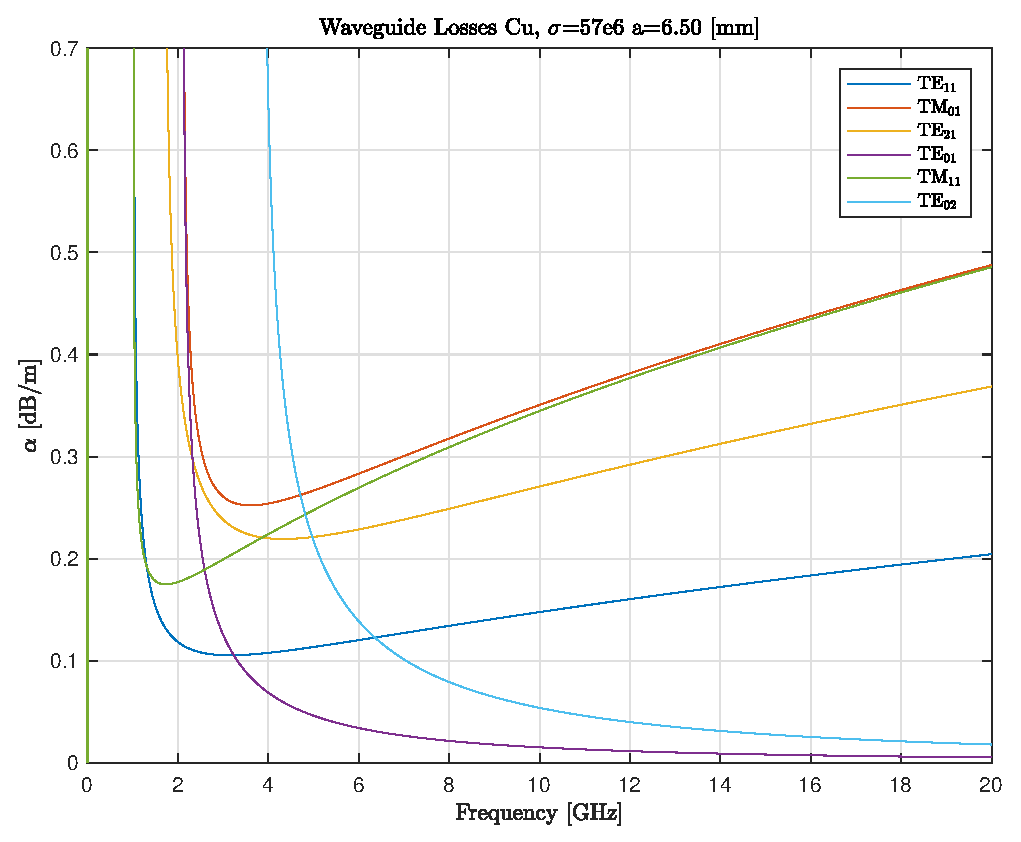
\includegraphics[width=\textwidth]{figures/wc13_attenuation}
      		\caption{Radius $r=\SI{6.5}{\milli\meter}$.}
      	\end{subfigure}
      	~
      	\begin{subfigure}[b]{0.48\textwidth}
      		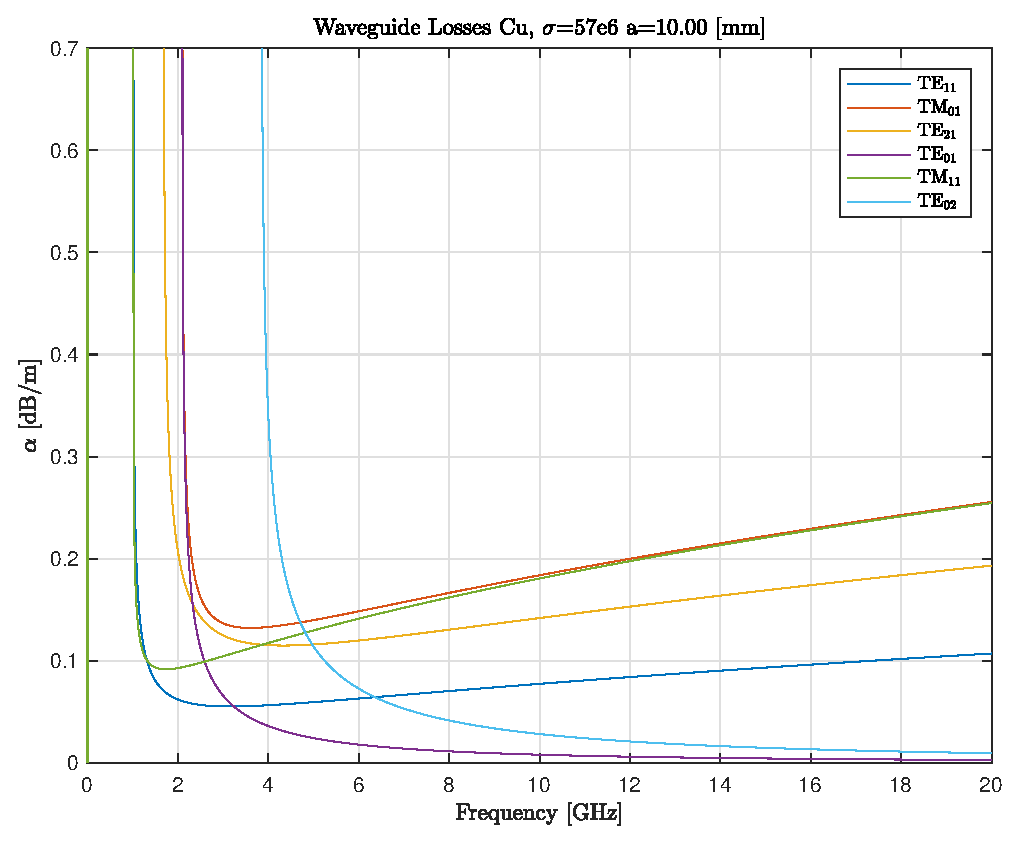
\includegraphics[width=\textwidth]{figures/wc20_attenuation}
      		\caption{Radius $r=\SI{10}{\milli\meter}$.}
      	\end{subfigure}
      	\caption{Waveguide attenuation for a circular waveguide of radius $r$ with copper conductor $\sigma=\SI{57e6}{\siemens\per\metre}$.}
      	\label{fig:wc_attenuation}
      \end{figure}
      
    
      \begin{table}[H]
        \centering		 
        \caption{Mode list for a circular waveguide with radius $r=\SI{6.5}{\milli\meter}$ without symmetry constraints.}
        \begin{tabular}{c|c|c|c|c}
          Mode number & Mode name & Cut-off frequency [GHz] & xz-symmetry & yz-symmetry\\
          \hline
          1 & TE\textsubscript{11c} & $\num{13.515}$ & EW & MW\\
          2 & TE\textsubscript{11s} & $\num{13.515}$ & MW & EW\\
          3 & TM\textsubscript{01} & $\num{17.653}$ & MW & MW\\
          4 & TE\textsubscript{21c} & $\num{22.420}$ & EW & EW\\
          5 & TE\textsubscript{21s} & $\num{22.420}$ & MW & MW\\
          6 & TE\textsubscript{01} & $\num{28.127}$ & EW & EW\\
          7 & TM\textsubscript{11c} & $\num{28.127}$ & MW & EW\\
          8 & TM\textsubscript{11s} & $\num{28.127}$ & EW & MW\\
          9 & TE\textsubscript{31c} & $\num{30.839}$ & EW & MW\\
          10 & TE\textsubscript{31s} & $\num{30.839}$ & MW & EW\\
          11 & TM\textsubscript{21c} & $\num{37.698}$ & MW & MW\\
          12 & TM\textsubscript{21s} & $\num{37.698}$ & EW & EW\\
          13 & TE\textsubscript{41c} & $\num{39.034}$ & EW & EW\\
          14 & TE\textsubscript{41s} & $\num{39.034}$ & MW & MW\\
          15 & TE\textsubscript{12c} & $\num{39.136}$ & EW & MW\\
          16 & TE\textsubscript{12s} & $\num{39.136}$ & MW & EW\\
          17 & TM\textsubscript{02} & $\num{40.520}$ & MW & MW\\
          18 & TM\textsubscript{31c} & $\num{46.834}$ & MW & EW\\
          19 & TM\textsubscript{31s} & $\num{46.834}$ & EW & MW\\
          20 & TE\textsubscript{51c} & $\num{47.094}$ & EW & MW\\
          21 & TE\textsubscript{51s} & $\num{47.094}$ & MW& EW\\
          22 & TE\textsubscript{22c} & $\num{49.227}$ & EW & EW\\
          23 & TE\textsubscript{22s} & $\num{49.227}$ & MW & MW			
        \end{tabular}
        \label{table:wc13}
      \end{table}
    
      \begin{table}[H]
        \centering		
        \caption{Mode list for a circular waveguide with radius $r=\SI{10}{\milli\meter}$ without symmetry constraints.}
        \begin{tabular}{c|c|c|c|c}
          Mode number & Mode name & Cut-off frequency [GHz] & xz-symmetry & yz-symmetry\\
          \hline
          1 & TE\textsubscript{11c} & $\num{8.7849}$ & EW & MW\\
          2 & TE\textsubscript{11s} & $\num{8.7849}$ & MW & EW\\
          3 & TM\textsubscript{01} & $\num{11.474}$ & MW & MW\\
          4 & TE\textsubscript{21c} & $\num{14.573}$ & EW & EW\\
          5 & TE\textsubscript{21s} & $\num{14.573}$ & MW & MW\\
          6 & TE\textsubscript{01} & $\num{18.282}$ & EW & EW\\
          7 & TM\textsubscript{11c} & $\num{18.282}$ & MW & EW\\	
          8 & TM\textsubscript{11s} & $\num{18.282}$ & EW & MW\\
          9 & TE\textsubscript{31c} & $\num{20.045}$ & EW & MW\\
          10 & TE\textsubscript{31s} & $\num{20.045}$ & MW & EW\\
          11 & TM\textsubscript{21c} & $\num{24.504}$ & MW & MW\\
          12 & TM\textsubscript{21s} & $\num{24.504}$ & EW & EW\\
          13 & TE\textsubscript{41c} & $\num{25.372}$ & EW & EW\\
          14 & TE\textsubscript{41s} & $\num{25.372}$ & MW & MW\\
          15 & TE\textsubscript{12c} & $\num{25.438}$ & EW & MW\\
          16 & TE\textsubscript{12s} & $\num{25.438}$ & MW & EW\\
          17 & TM\textsubscript{02} & $\num{26.338}$ & MW & MW\\
          18 & TM\textsubscript{31c} & $\num{30.442}$ & MW & EW\\
          19 & TM\textsubscript{31s} & $\num{30.442}$ & EW & MW\\
          20 & TE\textsubscript{51c} & $\num{30.611}$ & EW & MW\\
          21 & TE\textsubscript{51s} & $\num{30.611}$ & MW& EW\\
          22 & TE\textsubscript{22c} & $\num{31.997}$ & EW & EW\\
          23 & TE\textsubscript{22s} & $\num{31.997}$ & MW & MW		
        \end{tabular}
        \label{table:wc20}
      \end{table}
		
		
	
	\newpage
	\section{Designs and Results}
	\subsection{TEM coaxial mode to TE\textsubscript{10} rectangular waveguide mode transition}
		A waveguide transition between a \ac{SMA} coaxial connector and a rectangular waveguide (\ac{WR}75) with \ac{TE}\textsubscript{10} as the main transmitting mode is to be designed.\\
		
		The proposed design consists of the insertion of the connector into the waveguide by means of a termination in a metallic protuberance with the aim of improving the matching of the whole device.\\
		
		In this design the parameters of interest for the optimization are:
		\begin{itemize}
			\item Radius of the metallic protuberance $r_P$.
			\item Height of the metallic protuberance $h_P$.
			\item Length of the coaxial cable inserted into the waveguide $h_C$.
			\item Position of the coaxial connector with respect to the rectangular waveguide $z_C$. 
		\end{itemize}
		
		The position of the coaxial connector is constrained to be in the middle of the width of the rectangular waveguide and the protuberance is to have the same position with respect to the rectangular waveguide as the coaxial connector. No symmetries were found and thus not used in neither the simulation process nor the optimization process. The metallic protuberance helps the device to progressively transition from the \ac{TEM} mode from the coaxial cable to the final \ac{TE}\textsubscript{10} output gate mode. Some other designs with tuning screws were found but in this particular design, no tuning screws were necessary because of the excellent electromagnetic response of the device, having a return loss level higher than $\SI{20}{\decibel}$ resulting in a conversion efficiency higher than $\SI{99.7}{\percent}$ for the whole mono-mode recommended frequency band of the \ac{WR}75 waveguide ($\num{10}-\SI{15}{\giga\hertz}$, as stated in Table \ref{table:wr_dimensions}).\\
    
    The time-domain solver was used for both the simulation process and the optimization process due to the fact that there are not any resonant cavities and all the inserted energy is easily getting out of the structure, resulting in low convergence times. Plus, the structure is not complex (one of the simplest analyzed in this document), and low simulation times are thence obtained. \texttt{Trust Region Framework} was the used optimization method, and the final parameters values were easily obtained because of the limited number of optimization parameters.\\
    
    The main advantage of this design is the manufacturing process given the simplicity of it, for which the coaxial cable can be directly inserted into the rectangular waveguide due to the fact that the metallic protuberance located at the end of the aforementioned cable is in fact smaller than the necessary hole at the waveguide. Therefore, the metallic protuberance can be directly welded to the cable and the whole cable inserted into the previously made waveguide hole. However, both the position of the coaxial connector and especially the length of the coaxial cable inserted into the waveguide are extremely sensitive, i.e., a small change in the geometry could result in a high loss of conversion efficiency.\\
    
    Please note that given that proprietary connector designs are usually not publicly available, the coaxial connector is modelled as a simple coaxial cable, ignoring any return losses caused by itself.
		
		\begin{figure}[H]
			\centering
      
			\begin{subfigure}[b]{0.48\textwidth}
				\includegraphics[width=\textwidth]{figures/coaxToWaveguide}
				\caption{Scattering parameters.}
			\end{subfigure}
			~
			\begin{subfigure}[b]{0.48\textwidth}
				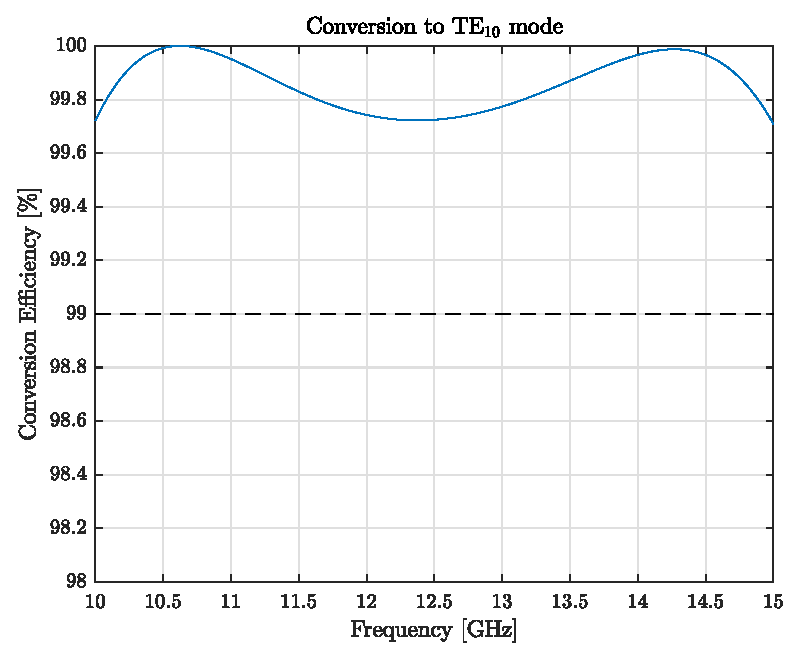
\includegraphics[width=\textwidth]{figures/coaxToWaveguide_eff}
				\caption{Conversion efficiency.}
			\end{subfigure}
		
			\caption{Scattering parameters results for the TEM coaxial mode to TE\textsubscript{10} rectangular waveguide mode transition.}
			\label{fig:coaxToWaveguide}
		\end{figure}
	
	
		\begin{figure}[H]
			\centering			
			\begin{subfigure}[b]{0.48\textwidth}
				\includegraphics[width=\textwidth]{renders/coaxToWaveguide}
			\end{subfigure}
			~
			\begin{subfigure}[b]{0.48\textwidth}
				\includegraphics[width=\textwidth]{renders/coaxToWaveguide-2}
			\end{subfigure}
			\vspace{10pt}\newline
			~
			\begin{subfigure}[b]{0.48\textwidth}
				\includegraphics[width=\textwidth]{renders/coaxToWaveguide-3}
			\end{subfigure}			
			\caption{TEM coaxial mode to TE\textsubscript{10} rectangular waveguide mode transition render.}
		\end{figure}
	
		\newpage
		\begin{landscape}
			\begin{figure}
				\centering
				\begin{subfigure}[b]{0.5\textwidth}
					\includegraphics[width=\textwidth]{figures/coaxToWaveguide_abs}
					\caption{Absolute value of electric field.}
				\end{subfigure}
				~ %add desired spacing between images, e. g. ~, \quad, \qquad, \hfill etc. 
				%(or a blank line to force the subfigure onto a new line)
				\begin{subfigure}[b]{0.5\textwidth}
					\includegraphics[width=\textwidth]{figures/coaxToWaveguide_lateral}
					\caption{Electric vector field. Lateral view.}
				\end{subfigure}
				\vspace{10pt}\newline
				~ %add desired spacing between images, e. g. ~, \quad, \qquad, \hfill etc. 
				%(or a blank line to force the subfigure onto a new line)
				\begin{subfigure}[b]{.7\textwidth}
					\includegraphics[width=\textwidth]{figures/coaxToWaveguide_front}
					\caption{Electric vector field. Front view.}
				\end{subfigure}
				\caption{TEM coaxial mode to TE\textsubscript{10} rectangular waveguide mode transition. Electric field monitor at $f=\SI{12.5}{\giga\hertz}$.}
				\label{fig:coaxToWaveguide_field}
			\end{figure}
		\end{landscape}
	
	\newpage
	\subsection{TEM coaxial mode to TE\textsubscript{20} rectangular waveguide mode transition}
		\subsubsection{Preliminary analysis}
		A waveguide transition between a \ac{SMA} coaxial cable and a rectangular waveguide (\ac{WR}75) with \ac{TE}\textsubscript{20} as the main transmitting mode is to be designed.\\	
		
		Given that wide bandwidth is not a key driver for this design, higher-order modes than the desired \ac{TE}\textsubscript{20} shall be ommited by restricting the simulation frequency band to $\SI{15.8}{\giga\hertz}-\SI{17.5}{\giga\hertz}$, considering one single mode at the input port (coaxial cable, \ac{TEM} mode) and three modes at the output port (\ac{TE}\textsubscript{10}, \ac{TE}\textsubscript{20} and \ac{TE}\textsubscript{01}).\\
		
		Please note that both \ac{TE}\textsubscript{01} and \ac{TE}\textsubscript{20} modes are degenerated modes with the same cut-off frequency, forcing the need of setting a polarization angle at the output port (in this case set to $\ang{0}$).
		
		\subsubsection{Design proposal I}
		In the present design proposed by \cite{montgomery}, shown in Figure \ref{fig:book_coax2wrte20_a}, the phase difference of $\ang{180}$ necessary to generate the \ac{TE}\textsubscript{20} mode is achieved by a geometrical contra-phase feeding at the waveguide. This way of feeding the \ac{TEM} mode form the coaxial cable to the waveguide is specially suitable for the desired output mode since the latter has a $\angle{180}$ phase difference at its maximum magnitude in two points (in which ideally the coaxial feeding structure should be placed) and this contra-phase feeding is used to achieve an outstanding mode purity because of the geometrical configuration of the other undesired modes, i.e. \ac{TE}\textsubscript{10} and \ac{TE}\textsubscript{01}.
		
		\begin{figure}[H]
			\centering
			\includegraphics[width=.5\textwidth]{figures/book_coax2wrte20_a}
			\caption{Proposed structure in \cite{montgomery} for a TEM coaxial mode to TE\textsubscript{20} rectangular waveguide mode transition.}
			\label{fig:book_coax2wrte20_a}
		\end{figure}
	
		In this design the parameters of interest for the optimization are:
		\begin{itemize}
			\item Radius of the metallic protuberance $r_P$.
			\item Height of the metallic protuberance $h_P$.			
			\item Length of the coaxial cables inserted into the waveguide $h_C$.
			\item Position of the coaxial cables with respect to the rectangular waveguide $z_C$. 
			\item Position of the common feeding cable junction $z_J$.
			\item Position of the coaxial cables with respect to the longitudinal axis of the rectangular waveguide $x_C$ and $-x_C$.
			\item Height of the coaxial cable inserted into the waveguide from the protuberance to the cable bending point of the feeder $h_F$.
		\end{itemize}
	
		Since the bandwidth obtained with the model described in the Figure \ref{fig:book_coax2wrte20_a} was very limited and since the achieved mode purity was excellent (next mode under $\SI{-58}{\decibel}$), the idea of using tuning screws came to mind in order to broaden the bandwidth. First, an optimization with two tuning screws was done and although a broader bandwidth was obtained, a four screws design was further optimized and the results were the best ones. The usage of these additional four screws (whose $x$ coordinates were constrained to the ones of the feeding coaxial cables) brought, though six additional parameters of interest:
		
		\begin{itemize}
			\item Radius of the first pair of screws $r_{S1}$.
			\item Height of the first pair of screws $h_{S1}$.
			\item Position of the first pair of screws with respect to the rectangular waveguide $z_{S1}$.
			\item Radius of the second pair of screws $r_{S2}$.
			\item Height of the second pair of screws $h_{S2}$.
			\item Position of the second pair of screws with respect to the rectangular waveguide $z_{S2}$.
		\end{itemize}
    
    This optimization was performed over the previously optimized design, but the achieved usable bandwidth was in fact poorer. Therefore, a further optimization was performed by taking into account all the  thirteen aforementioned geometrical parameters, firstly with a global optimization via \texttt{Genetic Algorithm} and finally with a local optimization via \texttt{Trust Region Framework}. It can be observed in Figure \ref{fig:coaxToWrTE20_field} that both the dimensions of the protuberances and the height and position of the feeding structure (as well as the coaxial cable inserted into the waveguide) are drastically different to accommodate the field configuration to the new tuning screws in order to get the desired TE\textsubscript{20} at the output gate of the waveguide.\\
    
    This design is an excellent example of the fact that when adding additional elements, the inter-dependencies between them and the original structure has to be brought into question and a separate optimization is not enough to reach the best response which the structure can actually provide.\\
	
	Taking into account the efficiency threshold set, a bandwidth of $BW=\SI{107}{\mega\hertz}$ is obtained for the design without screws ($\num{17.107}-\SI{17.214}{\giga\hertz}$, $\SI{0.62}{\percent}$ of band) and $BW=\SI{581}{\mega\hertz}$ for the design with tuning screws ($\num{16.655}-\SI{17.236}{\giga\hertz}$, $\SI{3.43}{\percent}$ of band).
	
		\newpage
		\begin{figure}[H]
			\centering
						
			\begin{subfigure}[b]{0.48\textwidth}
				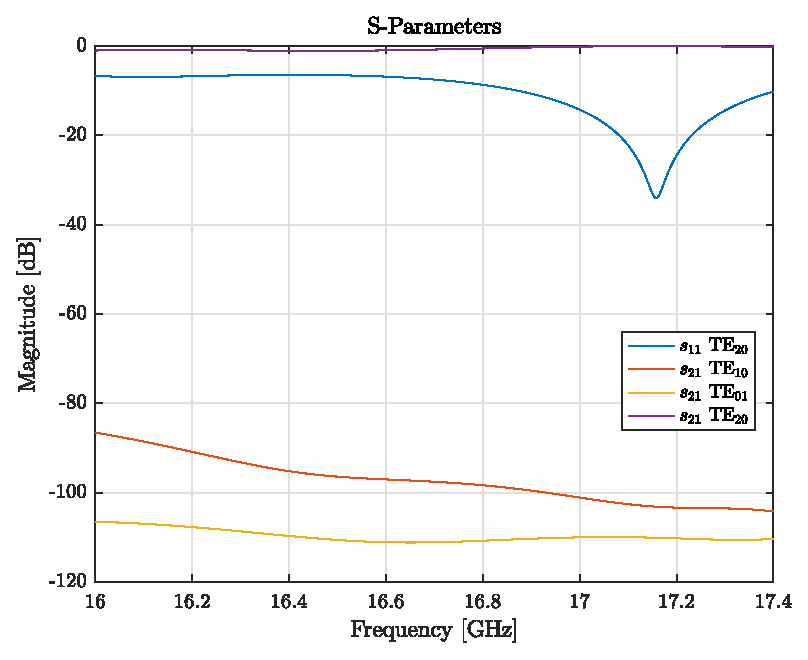
\includegraphics[width=\textwidth]{figures/coaxToWrTE20}
				\caption{Scattering parameters.}
			\end{subfigure}
			~
			\begin{subfigure}[b]{0.48\textwidth}
				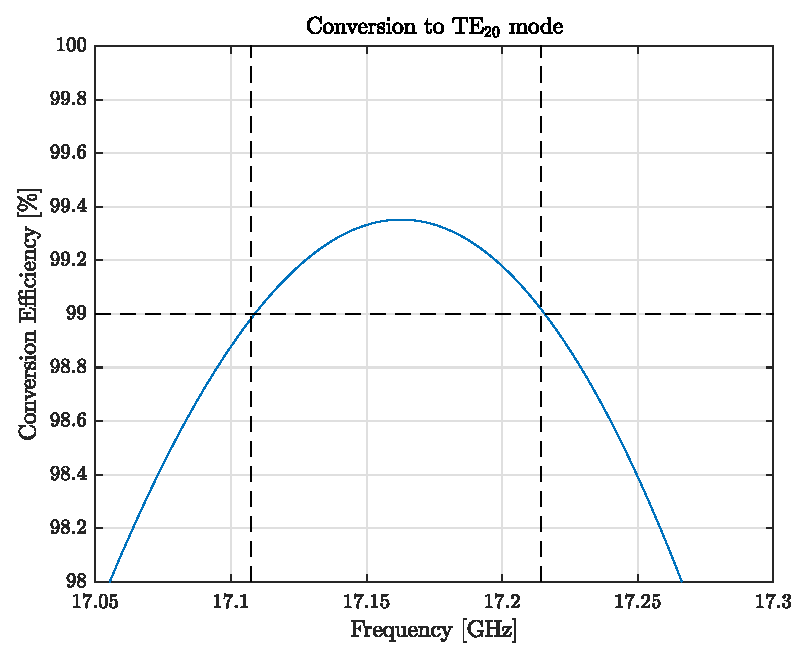
\includegraphics[width=\textwidth]{figures/coaxToWrTE20_eff}
				\caption{Conversion efficiency.}
			\end{subfigure}
		
			\caption{Results for the TEM coaxial mode to TE\textsubscript{20} rectangular waveguide mode transition Design I without tuning screws.}
			\label{fig:coaxToWrTE20}
		\end{figure}
	
		\begin{figure}[H]
			\centering
			\begin{subfigure}[b]{0.48\textwidth}
				\includegraphics[width=\textwidth]{figures/coaxToWrTE20_screw}
				\caption{Scattering parameters.}
			\end{subfigure}
			~
			\begin{subfigure}[b]{0.48\textwidth}
				\includegraphics[width=\textwidth]{figures/coaxToWrTE20_screw_eff}
				\caption{Conversion efficiency.}
			\end{subfigure}
		
			\caption{Results for the TEM coaxial mode to TE\textsubscript{20} rectangular waveguide mode transition Design I with tuning screws.}
			\label{fig:coaxToWrTE20_screw}
		\end{figure}
	
		\newpage
		\begin{figure}[H]
			\centering			
			\begin{subfigure}[b]{0.48\textwidth}
				\includegraphics[width=\textwidth]{renders/coaxToWrTE20_screw}
			\end{subfigure}
			~
			\begin{subfigure}[b]{0.48\textwidth}
				\includegraphics[width=\textwidth]{renders/coaxToWrTE20_screw-2}
			\end{subfigure}
			\vspace{10pt}\newline
			~
			\begin{subfigure}[b]{0.48\textwidth}
				\includegraphics[width=\textwidth]{renders/coaxToWrTE20_screw-3}
			\end{subfigure}		
			~
			\begin{subfigure}[b]{0.48\textwidth}
				\includegraphics[width=\textwidth]{renders/coaxToWrTE20_screw-4}
			\end{subfigure}	
			\caption{TEM coaxial mode to TE\textsubscript{20} rectangular waveguide mode transition Design I render.}
		\end{figure}	
	
		\newpage
		\begin{landscape}
			\begin{figure}
				\centering
				\begin{subfigure}[b]{0.4\textwidth}
					\includegraphics[width=\textwidth]{figures/coaxToWrTE20_abs}
					\caption{Absolute value of electric field.}
				\end{subfigure}
				~
				\begin{subfigure}[b]{0.4\textwidth}
					\includegraphics[width=\textwidth]{figures/coaxToWrTE20_front}
					\caption{Electric vector field. Front view.}
				\end{subfigure}
				\vspace{10pt}\\
				~ %add desired spacing between images, e. g. ~, \quad, \qquad, \hfill etc. 
				%(or a blank line to force the subfigure onto a new line)
				\begin{subfigure}[b]{0.4\textwidth}
					\includegraphics[width=\textwidth]{figures/coaxToWrTE20_lateral1}
					\caption{Electric vector field. Lateral view at pin 1.}
				\end{subfigure}
				~
				\begin{subfigure}[b]{0.4\textwidth}
					\includegraphics[width=\textwidth]{figures/coaxToWrTE20_lateral2}
					\caption{Electric vector field. Lateral view at pin 2.}
				\end{subfigure}
				\caption{TEM coaxial mode to TE\textsubscript{20} rectangular waveguide mode transition Design I without tuning screws. Electric field monitor at $f=\SI{17.2}{\giga\hertz}$.}
        \label{fig:coaxToWrTE20_field}
			\end{figure}
		\end{landscape}
	
			
		\newpage
		\begin{landscape}
			\begin{figure}
				\centering
				\begin{subfigure}[b]{0.4\textwidth}
					\includegraphics[width=\textwidth]{figures/coaxToWrTE20_screw_abs}
					\caption{Absolute value of electric field.}
				\end{subfigure}
				~
				\begin{subfigure}[b]{0.4\textwidth}
					\includegraphics[width=\textwidth]{figures/coaxToWrTE20_screw_front}
					\caption{Electric vector field. Front view.}
				\end{subfigure}
				\vspace{10pt}\\
				~
				\begin{subfigure}[b]{0.4\textwidth}
					\includegraphics[width=\textwidth]{figures/coaxToWrTE20_screw_lateral1}
					\caption{Electric vector field. Lateral view at pin 1.}
				\end{subfigure}
				~
				\begin{subfigure}[b]{0.4\textwidth}
					\includegraphics[width=\textwidth]{figures/coaxToWrTE20_screw_lateral2}
					\caption{Electric vector field. Lateral view at pin 2.}
				\end{subfigure}
				\caption{TEM coaxial mode to TE\textsubscript{20} rectangular waveguide mode transition Design I with tuning screws. Electric field monitor at $f=\SI{17.17}{\giga\hertz}$.}
			\end{figure}
		\end{landscape}
		
		\subsubsection{Design proposal II}
		
		In the present design the phase difference between the two pins inserted into the waveguide is achieved by a difference in paths of length $2 x_\mathrm{coax}$ according to the model proposed by \cite{montgomery}, as shown in Figure \ref{fig:book_coax2wrte20_b}.\\
		
		Such difference shall be the main parameter of design of the model, allowing the set-up to provide a maximum \ac{TE}\textsubscript{20} response in the desired band of interest, by minimizing both: the \ac{TE}\textsubscript{10} presence in the output waveguide and the matching parameter $s_{11}$ for the \ac{TE}\textsubscript{20} mode.\\
		
		It is important to remark that in the present design proposal the \ac{TE}\textsubscript{10} mode cannot be avoided for all frequencies since the phase difference cannot be $\theta=\ang{90}$ for the complete considered frequency band. For this reason, the optimization has been set to allow an acceptable conversion efficiency value throughout the $\SI{16.75}{\giga\hertz}-\SI{17.25}{\giga\hertz}$ frequency band ($f_0 = \SI{17}{\giga\hertz}$, $BW=\SI{500}{\mega\hertz}$, $\SI{2.94}{\percent}$ of band). Plus, if mode purity is a driver for the design of the device, this design shall be discarded since it cannot provide with a pure \ac{TE}\textsubscript{20} mode throughout any frequency band.
		
		\begin{figure}[H]
			\centering
			\includegraphics[width=.5\textwidth]{figures/book_coax2wrte20_b}
			\caption{Proposed structure in \cite{montgomery} for a TEM coaxial cable to a rectangular waveguide with mode TE\textsubscript{20} transition, alternative.}
			\label{fig:book_coax2wrte20_b}
		\end{figure}
	
		In this design the parameters of interest for the optimization are:
		\begin{itemize}
			\item Radius of the metallic protuberance $r_P$.
			\item Height of the metallic protuberance $h_P$.
			
			\item Radius of the screws $r_S$.
			\item Height of the screws $h_S$.
			\item Position of the screws with respect to the rectangular waveguide $z_S$.
			\item Position of the screws with respect to the longitudinal axis of the rectangular waveguide $x_S$ and $-x_S$.
			
			\item Length of the coaxial cables inserted into the waveguide $h_C$.
			\item Position of the coaxial cables with respect to the rectangular waveguide $z_C$. 
			\item Position of the coaxial cables with respect to the longitudinal axis of the rectangular waveguide $x_C$ and $-x_C$.
			\item Height of the coaxial cable inserted into the waveguide from the protuberance to the cable split of the feeder $h_F$.
		\end{itemize}
	
		In order to get an acceptable value of return loss, the usage of two tuning screws was necessary, allowing the design to provide a return loss level above $\SI{20}{\decibel}$ for a much broader bandwidth. In any case, the achieved mode purity was limited by the feeding architecture as described above and the optimization could not be only constrained to the return loss level but also having control of the undesired modes level.\\
		
		Taking into account the efficiency threshold set, a bandwidth of $BW=\SI{400}{\mega\hertz}$ is obtained for the design ($\num{16.825}-\SI{17.225}{\giga\hertz}, \SI{2.35}{\percent}$ of band).
	
		\begin{figure}[H]
			\centering			
			\begin{subfigure}[b]{0.48\textwidth}
				\includegraphics[width=\textwidth]{figures/coaxToWrTE20_alternative}
				\caption{Scattering parameters.}
			\end{subfigure}
			~
			\begin{subfigure}[b]{0.48\textwidth}
				\includegraphics[width=\textwidth]{figures/coaxToWrTE20_alternative_eff}
				\caption{Conversion efficiency.}
			\end{subfigure}
			\caption{Results for the TEM coaxial mode to TE\textsubscript{20} rectangular waveguide mode transition Design II with tuning screws.}
			\label{fig:coaxToWrTE20_alternative}
		\end{figure}
	
		\newpage
		\begin{figure}[H]
			\centering			
			\begin{subfigure}[b]{0.48\textwidth}
				\includegraphics[width=\textwidth]{renders/coaxToWrTE20_alternative}
			\end{subfigure}
			~
			\begin{subfigure}[b]{0.48\textwidth}
				\includegraphics[width=\textwidth]{renders/coaxToWrTE20_alternative-2}
			\end{subfigure}
			\vspace{10pt}\newline
			~
			\begin{subfigure}[b]{0.48\textwidth}
				\includegraphics[width=\textwidth]{renders/coaxToWrTE20_alternative-3}
			\end{subfigure}		
			\caption{TEM coaxial mode to TE\textsubscript{20} rectangular waveguide mode transition Design II render.}
		\end{figure}	

	
		\newpage
		\begin{landscape}
			\begin{figure}
				\centering
				\begin{subfigure}[b]{0.45\textwidth}
					\includegraphics[width=\textwidth]{figures/coaxToWrTE20_alternative_abs}
					\caption{Absolute value of electric field.}
				\end{subfigure}
				~
				\begin{subfigure}[b]{0.45\textwidth}
					\includegraphics[width=\textwidth]{figures/coaxToWrTE20_alternative_front}
					\caption{Electric vector field. Front view.}
				\end{subfigure}
				\vspace{10pt}\\
				~
				\begin{subfigure}[b]{0.45\textwidth}
					\includegraphics[width=\textwidth]{figures/coaxToWrTE20_alternative_lateral1}
					\caption{Electric vector field. Lateral view at pin 1.}
				\end{subfigure}
				~
				\begin{subfigure}[b]{0.45\textwidth}
					\includegraphics[width=\textwidth]{figures/coaxToWrTE20_alternative_lateral2}
					\caption{Electric vector field. Lateral view at pin 2.}
				\end{subfigure}
				\caption{TEM coaxial mode to TE\textsubscript{20} rectangular waveguide mode transition Design II with tuning screws. Electric field monitor at $f=\SI{17}{\giga\hertz}$.}
			\end{figure}
		\end{landscape}
	
	\newpage
	\subsection{TE\textsubscript{10} rectangular waveguide mode to TM\textsubscript{01} circular waveguide mode transducer}
	\subsubsection{Preliminary Analysis}
		A mode transducer between a rectangular waveguide (\ac{WR}75) and a circular waveguide with radius $r$ and \ac{TM}\textsubscript{01} as transmitting mode is to be designed.\\
		
		The first parameter to fix is the radius $r=\SI{10}{\milli\metre}$ to allow the TM\textsubscript{01} mode within the recommended frequency band of the \ac{WR}75 input waveguide. For this purpose, a suitable radius is chosen with the mode cut-off frequencies specified in Table \ref{table:wc20}.\\
				
		Taking into account the geometrical symmetry plane of both design proposals and the symmetry present at the input port (\ac{TE}\textsubscript{10} as only mode) at the rectangular waveguide and at the output port (\ac{TE}\textsubscript{01} as desired mode), the YZ plane can be defined as a magnetic wall (since both modes share the same magnetic wall symmetry), allowing much faster optimization by avoiding non-present modes computation and reducing the total meshing space by half. Theoretical modes with this symmetry are the ones in Table \ref{table:wc20_xm}, in the simulation frequency: \ac{TE}\textsubscript{11c} and \ac{TM}\textsubscript{01}.
		
		\begin{table}[H]
			\centering		
			\caption{Mode list for a circular waveguide with radius $r=\SI{10}{\milli\meter}$ with one magnetic wall.}
			\begin{tabular}{c|c|c|c|c}
				Mode number & Mode name & Cut-off frequency [GHz] & xz-symmetry & yz-symmetry\\
				\hline
				1 & TE\textsubscript{11c} & $\num{8.7849}$ & EW & MW\\
				2 & TM\textsubscript{01} & $\num{11.474}$ & MW & MW\\
				3 & TE\textsubscript{21s} & $\num{14.573}$ & MW & MW\\
				4 & TM\textsubscript{11s} & $\num{18.282}$ & EW & MW\\
				5 & TE\textsubscript{31c} & $\num{20.045}$ & EW & MW\\
				6 & TM\textsubscript{21c} & $\num{24.504}$ & MW & MW\\
				7 & TE\textsubscript{41s} & $\num{25.372}$ & MW & MW\\
				8 & TE\textsubscript{12c} & $\num{25.438}$ & EW & MW\\
				9 & TM\textsubscript{02} & $\num{26.338}$ & MW & MW\\
				10 & TM\textsubscript{31s} & $\num{30.442}$ & EW & MW\\
				11 & TE\textsubscript{51c} & $\num{30.611}$ & EW & MW\\
				12 & TE\textsubscript{22s} & $\num{31.997}$ & MW & MW		
			\end{tabular}
			\label{table:wc20_xm}
		\end{table}
	
		The present mode transducer will be designed with two different solutions, a design with irises and another with another intermediate circular waveguide and a coaxial with protuberances as the transmission medium between both the input rectangular waveguide and the output circular waveguide.
		
	\subsubsection{Design Proposal I}
		This mode transducer will be designed according to the proposal in \cite{montgomery} as showed in Figure \ref{fig:book_wr2wctm01}. In this case, the desired \ac{TM}\textsubscript{01} mode will be generated thanks to two symmetrical inductive irises which modify the field configuration at the intersection between the circular and the rectangular waveguide.\\
    
		\begin{figure}[H]
			\centering
			\includegraphics[width=.5\textwidth]{figures/book_wr2wctm01}
			\caption{Proposed structure in \cite{montgomery} for a rectangular waveguide with mode TE\textsubscript{10} to a circular waveguide with mode TM\textsubscript{01}.}
			\label{fig:book_wr2wctm01}
		\end{figure}
    
    As mentioned in \cite{montgomery}, the coupling can be achieved by meeting a matched condition avoiding the nearly total reflection, making usage of an impedance-matching element. In this case, this element is the symmetric iris which create a resonant cavity, having two major drawbacks:
    \begin{itemize}
        \item The matched condition is only met over a very narrow frequency range.
        \item The resistive losses and the electric field strength in the cavity would be greatly increased.
    \end{itemize}
    
    This last drawback can be observed in the Figure \ref{fig:wrToWcTM01_irises_field}, where the part of the structure having the highest value of electric field is precisely this cavity conformed between the irises and the waveguide junction. Apart from the physical disadvantages, the fact of having a resonant cavity causes the time-domain solver to be extremely slow due to the time required from the energy to escape the structure. This drawback is easily overcome by making usage of the frequency-domain solver, for which the required simulation time is reduced by a factor of almost 10 (from more than a minute to a few seconds).\\
	
		In this design the parameters of interest for the optimization are:
		\begin{itemize}
			\item Thick of the iris $t_I$.
			\item Width of the iris $w_I$.
			\item Position of the iris $z_I$.
			\item Position of the circular waveguide with respect to the rectangular waveguide $z_C$.
		\end{itemize}
		
		The position of the circular waveguide is constrained to be in the middle of the width of the rectangular waveguide and the symmetric iris is identical on either side to maintain the structure's plane of symmetry.\\
		
		Taking into account the efficiency threshold set, a bandwidth of $BW=\SI{813}{\mega\hertz}$ is obtained for the design ($\num{13.153}-\SI{13.966}{\giga\hertz}$, $\SI{6}{\percent}$ of band), as shown in the Figure \ref{fig:wrToWcTM01_irises}.
		
		\begin{figure}[H]
			\centering			
			\begin{subfigure}[b]{0.48\textwidth}
				\includegraphics[width=\textwidth]{figures/wrToWcTM01_irises}
				\caption{Scattering parameters.}
			\end{subfigure}
			~
			\begin{subfigure}[b]{0.48\textwidth}
				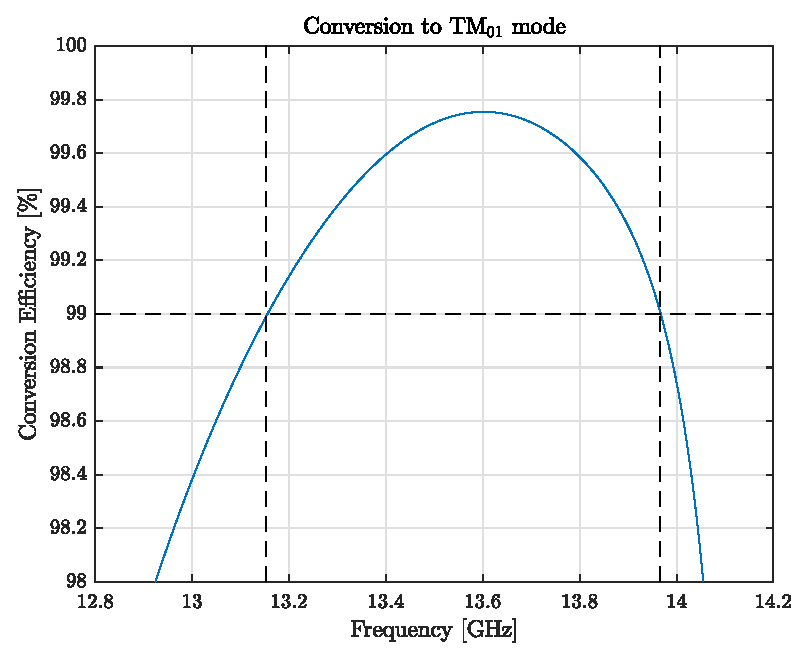
\includegraphics[width=\textwidth]{figures/wrToWcTM01_irises_eff}
				\caption{Conversion efficiency.}
			\end{subfigure}
			\caption{Results for the TE\textsubscript{10} rectangular waveguide mode to TM\textsubscript{01} circular waveguide mode transducer Design I.}
			\label{fig:wrToWcTM01_irises}
		\end{figure}
	
		\begin{figure}[H]
			\centering
			\includegraphics[width=.7\textwidth]{renders/wrToWcTM01_irises}
			\caption{TE\textsubscript{10} rectangular waveguide mode to TM\textsubscript{01} circular waveguide mode transducer Design I render.}
		\end{figure}
		
	
		\newpage
		\begin{landscape}
			\begin{figure}
				\centering
				\begin{subfigure}[b]{0.5\textwidth}
					\includegraphics[width=\textwidth]{figures/wrToWcTM01_irises_abs}
					\caption{Absolute value of electric field.}
				\end{subfigure}
				~
				\begin{subfigure}[b]{0.5\textwidth}
					\includegraphics[width=\textwidth]{figures/wrToWcTM01_irises_front}
					\caption{Electric vector field. Front view.}
				\end{subfigure}
				\vspace{10pt}\newline
				~
				\begin{subfigure}[b]{.7\textwidth}
					\includegraphics[width=\textwidth]{figures/wrToWcTM01_irises_lateral}
					\caption{Electric vector field. Lateral view.}
				\end{subfigure}
				\caption{TE\textsubscript{10} rectangular waveguide mode to TM\textsubscript{01} circular waveguide mode transducer Design I. Electric field monitor at $f=\SI{13.6}{\giga\hertz}$.}
        \label{fig:wrToWcTM01_irises_field}
			\end{figure}
		\end{landscape}
		
	\subsubsection{Design Proposal II}
		The present mode transducer will be designed with an own design consisting of an intermediate circular waveguide and a coaxial structure with a cylindrical dielectric with a metal cylinder inside terminated in two protuberances to maximize the transmitting ration to the desired mode of the final circular waveguide.\\
		
		In this design the parameters of interest for the optimization are:
		\begin{itemize}
			\item Length of the transitional circular waveguide $h_{C1}$.
			\item Radius of the transitional circular waveguide $r_{C1}$.
			\item Radius of the bottom metallic protuberance $r_{Pb}$.
			\item Height of the bottom metallic protuberance $h_{Pb}$.
			\item Radius of the top metallic protuberance $r_{Pt}$.
			\item Radius of the top metallic protuberance $h_{Pt}$.
			\item Height of the metallic core of the coaxial cable inserted into the rectangular waveguide from the protuberance to the nominal coaxial cable $h_{F1}$.
			\item Height of the metallic core of the coaxial cable inserted into the circular waveguide from the protuberance to the nominal coaxial cable $h_{F2}$.
			\item Radius of the tuning screw $r_S$.
			\item Height of the tuning screw $h_S$.
			\item Position of the tuning screw with respect to the rectangular waveguide $z_S$.
			\item Position of the circular waveguides with respect to the rectangular waveguide $z_C$.
		\end{itemize}
	
		Adding up to a total of twelve optimization parameters, the optimization process consisted of two parts: the optimization of the structure without the screws via global optimization (in this case \texttt{Genetic Algorithm}) and the optimization of the whole structure in order to get a better matching parameter with a local optimization method (\texttt{Trust Region Framework}).\\
		
		Taking into account the efficiency threshold set, a bandwidth of $BW=\SI{2037}{\mega\hertz}$ is obtained for the design ($\num{12.223}-\SI{14.260}{\giga\hertz}$, $\SI{15.38}{\percent}$ of band).\\

    Please note that the obtained useful bandwidth is about $\SI{250}{\percent}$ higher than the obtained with the design proposal I. but with the drawback of having a much more complex structure and with a likely much higher manufacturing cost given that the intermediate metallic part has to be mounted separately, i.e., the coaxial cable with the metallic protuberances cannot be directly inserted. However, the manufacturing process of the design proposal I is estimated to be much easier, having only the junction between both rectangular and circular waveguides and the irises in the interior of the rectangular waveguide.
		
		\begin{figure}[H]
			\centering			
			\begin{subfigure}[b]{0.48\textwidth}
				\includegraphics[width=\textwidth]{figures/wrToWcTM01}
				\caption{Scattering parameters.}
			\end{subfigure}
			~
			\begin{subfigure}[b]{0.48\textwidth}
				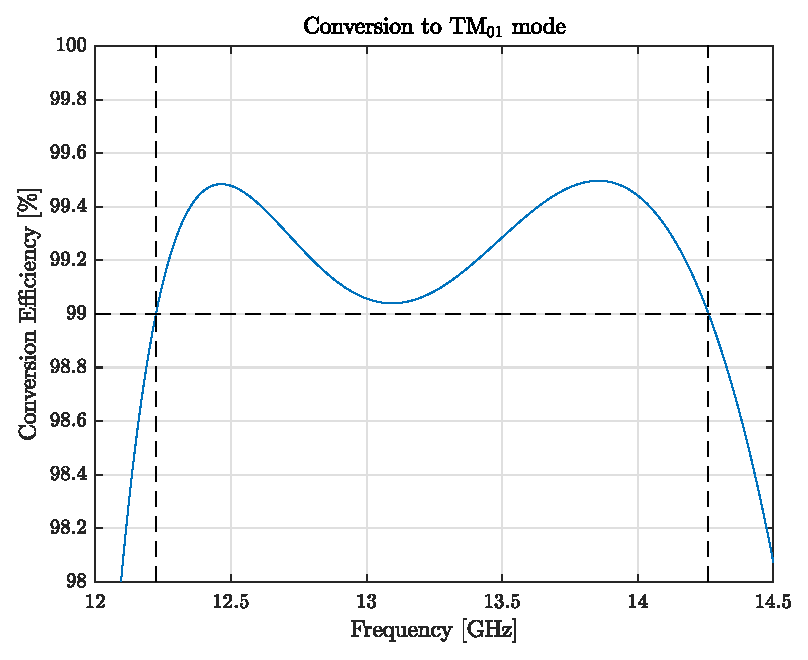
\includegraphics[width=\textwidth]{figures/wrToWcTM01_eff}
				\caption{Conversion efficiency.}
			\end{subfigure}
			\caption{Results for the TE\textsubscript{10} rectangular waveguide mode to TM\textsubscript{01} circular waveguide mode transducer Design II.}
			\label{fig:wrToWcTM01}
		\end{figure}
	
		\begin{figure}[H]
			\centering
			\includegraphics[width=.7\textwidth]{renders/wrToWcTM01}
			\caption{TE\textsubscript{10} rectangular waveguide mode to TM\textsubscript{01} circular waveguide mode transducer Design II render.}
		\end{figure}
	
		\newpage
		\begin{landscape}
			\begin{figure}
				\centering
				\begin{subfigure}[b]{0.45\textwidth}
					\includegraphics[width=\textwidth]{figures/wrToWcTM01_abs}
					\caption{Absolute value of electric field.}
				\end{subfigure}
				~
				\begin{subfigure}[b]{0.45\textwidth}
					\includegraphics[width=\textwidth]{figures/wrToWcTM01_front}
					\caption{Electric vector field. Front view.}
				\end{subfigure}
				\vspace{10pt}\newline
				~
				\begin{subfigure}[b]{.5\textwidth}
					\includegraphics[width=\textwidth]{figures/wrToWcTM01_lateral}
					\caption{Electric vector field. Lateral view.}
				\end{subfigure}
				\caption{TE\textsubscript{10} rectangular waveguide mode to TM\textsubscript{01} circular waveguide mode transducer Design II. Electric field monitor at $f=\SI{13.6}{\giga\hertz}$.}
				\label{fig:wrToWcTM01_field}
			\end{figure}
		\end{landscape}
		
	\newpage
	\subsection{TE\textsubscript{10} rectangular waveguide mode to TE\textsubscript{20} rectangular waveguide mode transducer}
    This waveguide mode transducer will be designed according to the proposal in \cite{montgomery} as showed in Figure \ref{fig:book_wr2wrte20}. The output \ac{TE}\textsubscript{20} mode shall be achieved by a resonant cavity formed by the symmetric iris and the waveguide junction, conforming accordingly the mode geometry for the desired frequency band at the output gate. The principle of operation is identical to the previously studied \ac{TE}\textsubscript{10} rectangular waveguide mode to \ac{TM}\textsubscript{01} circular waveguide mode transducer Design I, causing the same physical and simulating difficulties. That is the reason why the frequency-domain solver was accordingly used in order to reduce the computation time.
  
		\begin{figure}[H]
			\centering
			\includegraphics[width=.5\textwidth]{figures/book_wr2wrte20}
			\caption{Proposed structure in \cite{montgomery} for a rectangular waveguide with mode TE\textsubscript{10} to a rectangular waveguide with mode TE\textsubscript{20}.}
			\label{fig:book_wr2wrte20}
		\end{figure}
	
		In this design the parameters of interest for the optimization are:
		\begin{itemize}
			\item Thick of the iris $t_I$.
			\item Width of the iris $w_I$.
			\item Position of the iris $z_I$.
			\item Position of the output rectangular waveguide with respect to the input rectangular waveguide $z_{RO}$
		\end{itemize}
    
    The height of the irises is set to cover the whole height of the waveguide, i.e. $h_I=b$.\\
    
    The design and optimization process has resulted in a structure whose complexity would allow the manufacturing by different techniques. As for the classical milling, it could be easily fabricated by dividing the structure into an upper and lower part and then joining them. This design would be also suitable for more innovative techniques such as Additive Manufacturing, in which the same division shall be performed and a vertical addition process would be easy and effective to implement. Nonetheless, although easily manufacturable, this design present two major drawbacks: narrow-band response and poor mode purity, which was expected because of its simplicity: the residual \ac{TE}\textsubscript{10} mode of the input port is, although attenuated, present at the output port with a minimum value of the transmission parameter in the band of interest of $\SI{-21.5}{\decibel}$.\\
	
		Taking into account the efficiency threshold set, a bandwidth of $BW=\SI{126}{\mega\hertz}$ is obtained for the design ($\num{16.285}-\SI{16.410}{\giga\hertz}$, $\SI{0.765}{\percent}$ of band) as shown in the Figure \ref{fig:wrToWrTE20}.\\
    
    The obtained bandwidth has, as explained for the previous design, a narrow-band response because of the resonant cavity described before. As a matter of example for comparison, when taking the \ac{TEM} coaxial mode to \ac{TE}\textsubscript{20} rectangular waveguide mode transition, a bandwidth about five times higher is obtained for the same mode at the identical output gate with a drastically higher mode purity ($\SI{-21.5}{\decibel}$ vs. $\SI{-58}{\decibel}$ of the transmission parameter of the strongest undesired mode).
	
		\begin{figure}[H]
			\centering			
			\begin{subfigure}[b]{0.48\textwidth}
				\includegraphics[width=\textwidth]{figures/wrToWrTE20_irises}
				\caption{Scattering parameters.}
			\end{subfigure}
			~
			\begin{subfigure}[b]{0.48\textwidth}
				\includegraphics[width=\textwidth]{figures/wrToWrTE20_irises_eff}
				\caption{Conversion efficiency.}
			\end{subfigure}
			\caption{Results for the TE\textsubscript{10} rectangular waveguide mode to TE\textsubscript{20} rectangular waveguide mode transducer.}
			\label{fig:wrToWrTE20}
		\end{figure}
	
		\begin{figure}[H]
			\centering
			\includegraphics[width=.7\textwidth]{renders/wrToWrTE20_irises}
			\caption{TE\textsubscript{10} rectangular waveguide mode to TE\textsubscript{20} rectangular waveguide mode transducer render.}
		\end{figure}
	
		\newpage
		\begin{landscape}
			\begin{figure}
				\centering
				\begin{subfigure}[b]{0.45\textwidth}
					\includegraphics[width=\textwidth]{figures/wrToWrTE20_input}
					\caption{Absolute value of electric field.}
				\end{subfigure}
				~
				\begin{subfigure}[b]{0.45\textwidth}
					\includegraphics[width=\textwidth]{figures/wrToWrTE20_output}
					\caption{Electric vector field. Front view.}
				\end{subfigure}
				\vspace{10pt}\newline
				~
				\begin{subfigure}[b]{.6\textwidth}
					\includegraphics[width=\textwidth]{figures/wrToWrTE20_abs}
					\caption{Electric vector field. Lateral view.}
				\end{subfigure}
				\caption{TE\textsubscript{10} rectangular waveguide mode to TE\textsubscript{20} rectangular waveguide mode transducer. Electric field monitor at $f=\SI{16.35}{\giga\hertz}$.}
				\label{fig:wrToWrTE20_abs}
			\end{figure}
		\end{landscape}
	
	\newpage
	\subsection{TE\textsubscript{20} rectangular waveguide mode to TE\textsubscript{01} circular waveguide mode transducer}
	 \begin{wrapfigure}{o}{.3\textwidth}
		\centering
		\includegraphics[width=.3\textwidth]{figures/wrTE20ToWcTE01_section}
		\caption{Section of the TE\textsubscript{20} rectangular waveguide mode to TE\textsubscript{01} circular waveguide mode transducer.}
		\label{fig:wrTE20ToWcTE01_section}
	\end{wrapfigure}
	
    This waveguide transition will be designed according to the proposal in \cite{montgomery} as showed in Figure \ref{fig:book_wrTE20ToWcTE01}. In this case, the theoretical idea is the progressive transformation of the input \ac{TE}\textsubscript{20} mode geometry to the final \ac{TE}\textsubscript{01} by adapting the structure geometry to the mode geometry making usage of a tapered transition. Theoretically, in the case of tapered transitions where no inductive element is used to meet the matching condition, a broader bandwidth is to be expected and since the change is gradual, the propagation occurs with very little reflection.\\
    
   
    
    However, the proposed structure is not directly defined but only through intermediate sections, whose dimensions are not specified. Because of this reason, several intermediate sections are defined with curves and then joined by the CAD software with the tapering tool.\\
    
    The motivation of this waveguide transition is taking advantage of the fact that the \ac{TE}\textsubscript{01} circular waveguide mode is the one providing less attenuation per unit of length of the whole set analysed as previously shown in Figure \ref{fig:wc_attenuation}. This advantage would be of particular interest in applications where low losses are desired, for instance the transportation of high power over a long structure. Plus, the attenuation for this mode is a monotonically decreasing, in contrast to the fundamental \ac{TE}\textsubscript{11} mode, allowing for a low-loss power transfer over an unlimited bandwidth (only limited by the presence of higher modes). \\ 
    
    
    
    Through a preliminary analysis of the proposed structure, the presence of two geometrical symmetry planes is easily observed and this fact was extremely useful in the simulation and further optimization given that both input and output desired modes share the same electrical symmetries, i.e., xz- and yz-electrical walls, allowing for the simulation of only one fourth of the total structure and constraining the mode presence to the ones compliant with the established symmetry: only the \ac{TE}\textsubscript{20} at the input gate and \ac{TE}\textsubscript{21c} and \ac{TE}\textsubscript{01} for frequencies under $\SI{24.5}{\giga\hertz}$ (as showed in Tables \ref{table:wc20_ee} and \ref{table:wr75_ee_modes}). Therefore, the output circular waveguide radius was chosen in order for the \ac{TE}\textsubscript{01} mode to have a higher cut-off frequency than the input \ac{TE}\textsubscript{20} (fixed by the WR75 dimensions) but lower than the cut-off frequency of the next mode in the rectangular waveguide taking into account the symmetries ($\SI{31.474}{\giga\hertz}$).\\
                
    
    
    In this design the parameters of interest for the optimization are:
    \begin{itemize}
      \item Radius of each of the intermediate circular section $r_{i}$.
      \item Height from which the angle of each of the intermediate section is defined $h_{i}$.
      \item Angle of aperture of the incision of each of the intermediate sections $\alpha_{i}$.
      \item Length between intermediate sections $L_i$.
      \item Blending parameter of the metallic incision $b_I$.
    \end{itemize}      
	
    A total of four sections have been taken into consideration for the design and optimization, resulting in a total amount of eighteen parameters: twelve parameters (radius, height and angle for each section) plus five lengths between sections and one blending parameter.\\
    
    Although the number of optimization parameters is high, a global optimization was possible due to the aforementioned symmetries and a further local optimization.
    
    \begin{figure}[H]
			\centering
			\includegraphics[width=.7\textwidth]{figures/book_wrTE20ToWcTE01}
			\caption{Proposed structure in \cite{montgomery} for a rectangular waveguide with mode TE\textsubscript{20} to a circular waveguide with mode TE\textsubscript{01}.}
			\label{fig:book_wrTE20ToWcTE01}
		\end{figure}
  
		\begin{table}[H]
			\centering		
			\caption{Mode list for a circular waveguide with radius $r=\SI{10}{\milli\meter}$ with both electrical walls.}
			\begin{tabular}{c|c|c|c|c}
				Mode number & Mode name & Cut-off frequency [GHz] & xz-symmetry & yz-symmetry\\
				\hline
				1 & TE\textsubscript{21c} & $\num{14.573}$ & EW & EW\\
				2 & TE\textsubscript{01} & $\num{18.282}$ & EW & EW\\
				3 & TM\textsubscript{21s} & $\num{24.504}$ & EW & EW\\
				4 & TE\textsubscript{41c} & $\num{25.372}$ & EW & EW\\
				5 & TE\textsubscript{22c} & $\num{31.997}$ & EW & EW\\	
			\end{tabular}
			\label{table:wc20_ee}
		\end{table}
	
		\begin{table}[H]
			\centering
			\caption{Mode list for WR75 with both electrical walls.}
			\begin{tabular}{c|c|c|c|c}
				Mode no. & Mode name & Cut-off frequency [GHz] & xz-symmetry & yz-symmetry\\
				\hline
				1 & TE\textsubscript{20} & $\num{15.737}$ & EW & EW\\
				2 & TE\textsubscript{40} & $\num{31.474}$ & EW & EW\\
				3 & TE\textsubscript{02} & $\num{31.474}$ & EW & EW
			\end{tabular}
			\label{table:wr75_ee_modes}
		\end{table}
    
    Taking into account the efficiency threshold set, a bandwidth of $BW=\SI{342}{\mega\hertz}$ is obtained for the design ($\num{22.769}-\SI{23.111}{\giga\hertz}$, $\SI{1.49}{\percent}$ of band).
    
    \begin{figure}[H]
		\centering			
		\begin{subfigure}[b]{0.48\textwidth}
			\includegraphics[width=\textwidth]{figures/wrTE20ToWcTE01}
			\caption{Scattering parameters.}
		\end{subfigure}
		~
		\begin{subfigure}[b]{0.48\textwidth}
			\includegraphics[width=\textwidth]{figures/wrTE20ToWcTE01_eff}
			\caption{Conversion efficiency.}
		\end{subfigure}
		\caption{Results for the TE\textsubscript{20} rectangular waveguide mode to TE\textsubscript{01} circular waveguide mode transducer.}
		\label{fig:wrTE20ToWcTE01}
	\end{figure}
	
	\begin{figure}[H]
		\centering
		\includegraphics[width=.7\textwidth]{renders/wrTE20ToWcTE01-2}
		\caption{TE\textsubscript{20} rectangular waveguide mode to TE\textsubscript{01} circular waveguide mode transducer render.}
	\end{figure}
    
    \newpage
		\begin{landscape}
			\begin{figure}
				\centering
				\begin{subfigure}[b]{0.6\textwidth}
					\includegraphics[width=\textwidth]{figures/wrTE20ToWcTE01_abs}
					\caption{Absolute value of electric field.}
				\end{subfigure}
				~
				\begin{subfigure}[b]{0.45\textwidth}
					\includegraphics[width=\textwidth]{figures/wrTE20ToWcTE01_output}
					\caption{Electric vector field. Front view.}
				\end{subfigure}
				\vspace{10pt}\newline
				~
				\begin{subfigure}[b]{.6\textwidth}
					\includegraphics[width=\textwidth]{figures/wrTE20ToWcTE01_lateral}
					\caption{Electric vector field. Lateral view.}
				\end{subfigure}
				\caption{TE\textsubscript{20} rectangular waveguide mode to TE\textsubscript{01} circular waveguide mode transducer. Electric field monitor at $f=\SI{23.0}{\giga\hertz}$.}
			\end{figure}
		\end{landscape}
	
		
	
	\newpage
	\subsection{TE\textsubscript{10} rectangular waveguide mode to TE\textsubscript{01} circular waveguide mode transducer}
    Within the category of the aforementioned tapered mode transducers in which a gradual geometry change is induced (also called flared-type), a \ac{TE}\textsubscript{10} rectangular waveguide mode to \ac{TE}\textsubscript{01} circular waveguide mode transducer is to be designed.\\
    
    \begin{wrapfigure}{o}{.3\textwidth}
    	\centering
    	\includegraphics[width=.3\textwidth]{figures/marie_plano}
    	\caption{Section of the TE\textsubscript{10} rectangular waveguide mode to TE\textsubscript{01} circular waveguide mode transducer.}
    	\label{fig:marie_plano}
    \end{wrapfigure}
    
    As shown in the Figure \ref{fig:wc_attenuation} and previously discussed, the \ac{TE}\textsubscript{01} mode is especially suitable for a large variety of microwave engineering applications with the main goal of having low losses when the conductor is not perfect, due to its appropriate attenuation per unit of length and because of this attenuation being monotonically decreasing as the frequency increases, for instance low loss filters, plasma-heating devices (in which resonators with high Q-factors in cavity filters or high energy systems are implemented, e.g. \cite{blank}, \cite{leou}), long transmission systems or power combining devices (in which this sort of transitions allow for a more efficient power handling and extension to other frequencies, \cite{chen}) to mention but a few. \\

	Traditionally, there have been two ways in order to achieve this mode transformation: by basing the design on the sidewall coupling between both input and output waveguides (\cite{nusinovich}) or by basing it on slowly flared structures with different cross-sections (e.g. the final implemented structure in this document), taking advantage of certain symmetries to prevent the higher-mode generation.\\
    
    The design of this device had to cope with a very broad bandwidth covering the complete Q-band (i.e. $\num{33}-\SI{50}{\giga\hertz}$) and to provide an acceptable level of both matching (under $\SI{-20}{\decibel}$) and mode purity. As a reference, the Marié slowly flared structure (\cite{saad}, \cite{marie}) was taken into consideration because of its bandwidth and mode purity capabilities. However, this structure requires for the simulation 23 modes at the output circular waveguide to be taken into account (Table \ref{table:wc13}) and this fact presents a non-avoidable computational cost.\\
    
    The possibility of using an electric wall along the xz plane given the input and output desired modes (\ac{TE}\textsubscript{10} and \ac{TE}\textsubscript{01}) makes the usage of only 11 modes possible (Table \ref{table:wc13_ex}), dramatically reducing the computation time as long as improving the mode purity (avoiding the modes which are non-compliant to this electrical wall restriction). Nonetheless, computation time is still a key driver for the further optimization, in which the high number of optimization parameters and the lack of proper simulation hardware makes a global optimization with all the parameters infeasible given the high processing cost of not only obtaining both the electric and magnetic field in each simulation cell of the full-wave analysis but also projecting both fields at the input and output device gates in the mode auto-functions to evaluate the optimization cost functions via the scattering parameters for each of the modes of interest.\\
    
    \begin{table}
        \centering		 
        \caption{Mode list for a circular waveguide with radius $r=\SI{6.5}{\milli\meter}$ with electrical wall xz-symmetry.}
        \begin{tabular}{c|c|c|c|c}
          Mode number & Mode name & Cut-off frequency [GHz] & xz-symmetry & yz-symmetry\\
          \hline
          1 & TE\textsubscript{11c} & $\num{13.515}$ & EW & MW\\
          2 & TE\textsubscript{21c} & $\num{22.420}$ & EW & EW\\
          3 & TE\textsubscript{01} & $\num{28.127}$ & EW & EW\\
          4 & TM\textsubscript{11s} & $\num{28.127}$ & EW & MW\\
          5 & TE\textsubscript{31c} & $\num{30.839}$ & EW & MW\\
          6 & TM\textsubscript{21s} & $\num{37.698}$ & EW & EW\\
          7 & TE\textsubscript{41c} & $\num{39.034}$ & EW & EW\\
          8 & TE\textsubscript{12c} & $\num{39.136}$ & EW & MW\\
          9 & TM\textsubscript{31s} & $\num{46.834}$ & EW & MW\\
          10 & TE\textsubscript{51c} & $\num{47.094}$ & EW & MW\\
          11 & TE\textsubscript{22c} & $\num{49.227}$ & EW & EW\\	
        \end{tabular}
        \label{table:wc13_ex}
      \end{table}
    
    The design purpose made in \cite{saad} has been modeled in the CAD editor from the \texttt{CST Studio Suite} software, implementing the different sections of the mode transducer. Nevertheless, the geometry specified in the aforementioned article is not completely defined and it is crucial to note that several design alternatives are possible for this device. In this case, neither the lengths of the different sections and taper parameters nor the exact intermediate sections were clearly specified and it is the labor of the final implementer to decide and conduct a proper optimization.\\
    
    As mentioned before, the optimization process cannot be conducted for all the possible parameters (whose number is above 20) due to the extremely high computational cost given the high number of modes to be taken into account for the simulation and therefore only the lengths of the different sections and tapers between sections have been optimized. The number of modes considered at the input port is 11 and, at the output port only one due to the fact that the \ac{WR}22 waveguide was used as the input gate, having the cut-off frequency of the next mode at $\SI{52.692}{\giga\hertz}$ corresponding to the \ac{TE}\textsubscript{20} mode, above the simulation frequency band.\\
    
    The structure consists of three main sections with an input \ac{WR}22 rectangular waveguide and an output circular waveguide with $r=\SI{13}{\milli\metre}$, joined between them with different tapers. The first section is in charge of converting the input rectangular waveguide \ac{TE}\textsubscript{10} mode to the rectangular \ac{TE}\textsubscript{20} mode, the second converts the rectangular waveguide to the X-cross-section circular waveguide and the third one converts this cross-section to the final circular waveguide.\\
    
    Since the in depth theoretical analysis of this device is out of the scope of the present document, more details can be found in the patent for the Marié-type transducer \cite{marie}.\\
    
    \begin{figure}
	      \centering
	      \includegraphics[width=.7\textwidth]{figures/marie_structure}
	      \caption{CAD model of the TE\textsubscript{10} rectangular waveguide mode to TE\textsubscript{01} circular waveguide mode transducer.}
	      \label{fig:marie_cad}
    \end{figure}
    
    \begin{figure}
			\centering			
			\begin{subfigure}[b]{0.48\textwidth}
				\includegraphics[width=\textwidth]{figures/marie_cst_transmission}
				\caption{Transmission.}
			\end{subfigure}
			~
			\begin{subfigure}[b]{0.48\textwidth}
				\includegraphics[width=\textwidth]{figures/marie_cst_eff}
				\caption{Conversion efficiency.}
			\end{subfigure}
		
		    \vspace{10pt}
		    
		      \begin{subfigure}[b]{0.48\textwidth}
				\includegraphics[width=\textwidth]{figures/marie_cst_matching}
				\label{fig:marie_cst_matching}
				\caption{Matching.}
			\end{subfigure}
			~
			\begin{subfigure}[b]{0.48\textwidth}
				\includegraphics[width=\textwidth]{figures/marie_cst_superior_modes}
				\label{fig:marie_cst_superior_modes}
				\caption{Higher-order modes transmissions.}
			\end{subfigure}
			\caption{Results for the TE\textsubscript{10} rectangular waveguide mode to TE\textsubscript{01} circular waveguide mode transducer. Lossless simulated structure}
			\label{fig:marie_cst}
		\end{figure}
    
    As shown in the Figure \ref{fig:marie_cst} (c), the lossless simulated structure provides a matching better than $\SI{-20}{\decibel}$ for the complete Q-band ($\SI{41}{\percent}$ relative bandwidth), achieving the initial goal of this design. In the Figure \ref{fig:marie_cst} (d) the transmission coefficient for the other ten propagating modes in the band of interest is depicted, all of them limited by $\SI{-45}{\decibel}$ except for \ac{TE}\textsubscript{41} mode reaching the value of $\SI{-25}{\decibel}$ at the very end of the band, but still under acceptable values. Furthermore, as stated in \cite{saad}, the \ac{TE}\textsubscript{41} mode can be easily eliminated via a helix mode filter with a negligible increase in loss for the desired \ac{TE}\textsubscript{01} mode.\\
    
    Once the design, optimization and analysis of the final structure was performed, different alternatives for the prototyping were analysed. Due to the length of the device, the manufacturing of such a long structure by traditional means would be in some cases unaffordable and thence, other alternatives were carefully examined, such as the new \ac{AM} technologies, which, although presenting some major drawbacks (mainly the fabrication precision), its extremely competitive price make them an option to analyse.\\
    
    Given the aforementioned main drawback of the fabrication precision presented by the \ac{AM} technologies, the prototyping of this device was a daunting challenge to overcome taking into account the fact that the recommended frequency band was the complete Q-band, in which the highest frequency has a wavelength in vacuum of $\lambda_0\approx\SI{6}{\milli\metre}$ and the usage of this technology is still under research. However, the geometry studied in this design is especially well suited for \ac{SLS} as further proved in the measured results \cite{gonzalez} and therefore this technology was to be employed in the prototyping process.\\
    
    In order to conduct the measurement process, both insertion loss and return loss have been measured in a back-to-back configuration owing to the simplicity of the measurement, for which two identical transducers were prototyped via \ac{SLS} using AlSi10Mg as main material. In the back-to-back configuration, a variable angular rotation is induced between both devices, in this case $\ang{0}$, $\ang{45}$, $\ang{90}$ and $\ang{180}$ as it can be observed in the Figure \ref{fig:marie_photo}, performing the measurement by connecting the device with the \ac{VNA} through two identical coaxial to \ac{WR}22 transitions.\\
    
	\begin{figure}
    	\centering			
    	\begin{subfigure}[b]{0.48\textwidth}
    		\includegraphics[width=\textwidth]{figures/marie_photo_45}
    		\caption{Measurement at $\ang{45}$.}
    	\end{subfigure}
    	~
    	\begin{subfigure}[b]{0.48\textwidth}
    		\includegraphics[width=\textwidth]{figures/marie_photo_90}
    		\caption{Measurement at $\ang{90}$.}
    	\end{subfigure}
    	\vspace{10pt}\\
    	\begin{subfigure}[b]{0.48\textwidth}
    		\includegraphics[width=\textwidth]{figures/marie_photo_0}
    		\caption{Measurement at $\ang{0}$.}
    	\end{subfigure}
    	\caption{Measurement in back-to-back configuration for different angular rotations of the TE\textsubscript{10} rectangular waveguide mode to TE\textsubscript{01} circular waveguide mode transducer \cite{gonzalez}.}
    	\label{fig:marie_photo}
    \end{figure}

	\begin{figure}
		\centering
		\includegraphics[width=.7\textwidth]{renders/Conversor_Marie_Prodintec_optimizado_stp}
		\caption{TE\textsubscript{20} rectangular waveguide mode to TE\textsubscript{01} circular waveguide mode transducer render.}
	\end{figure}

	With the goal of drawing a comparison between the simulated and measured results, a simulation with both devices with $\ang{0}$ angular rotation was performed by considering an effective electrical conductivity of $\sigma_\mathrm{eff}=\SI{2.1}{\mega\siemens\per\metre}$, taking into account the prototyping material properties, i.e. aluminium powder, as well as the roughness of the walls and the manufacturing process. Both the simulated and the measured results for matching ($s_{11}$) and transmission ($s_{21}$) scattering parameters are shown in the Figures \ref{fig:marie_measured} (c) and \ref{fig:marie_measured} (a).\\
    

	\begin{figure}
		\centering			
		\begin{subfigure}[b]{0.48\textwidth}
			\includegraphics[width=\textwidth]{figures/marie_measured_transmission}
			\caption{Transmission.}
		\end{subfigure}	
		~
		\begin{subfigure}[b]{0.48\textwidth}
			\includegraphics[width=\textwidth]{figures/marie_measured_eff}
			\caption{Conversion Efficiency.}
		\end{subfigure}
		\vspace{10pt}\\		
		\begin{subfigure}[b]{0.48\textwidth}
			\includegraphics[width=\textwidth]{figures/marie_measured_matching}
			\caption{Matching.}
		\end{subfigure}
		\caption{Results for the TE\textsubscript{10} rectangular waveguide mode to TE\textsubscript{01} circular waveguide mode transducer. Measured and lossy simulated structure.}
		\label{fig:marie_measured}
	\end{figure}

	Conversion efficiency is computed:
	
	\begin{equation}
		\textrm{CE}[\%]=100\cdot |s_{21}^{\textrm{b2b}}|
	\end{equation}	
	%
	where $s_{21}^{\textrm{b2b}}$ is the measured transmission parameter in the back-to-back configuration.\\    
	
	Figure \ref{fig:marie_measured} (c) shows the matching of both the simulated and measured structures, in which it can be seen that the matching parameter is mainly below $\SI{-20}{\decibel}$ for the complete band except for some frequencies. Nonetheless, the most interesting comparison comes with the Figure \ref{fig:marie_measured} (a), in which the matching between the simulated and the measured values is very promising easily checked by the superimposition of the curves onto each other. According to the conversion efficiency previously provided, Figure \ref{fig:marie_measured} (b) shows the conversion efficiency for the desired mode, in which the worst measured value is $\SI{83}{\percent}$ for the whole Q-band. These curves proves that excellent results can be provided by the \ac{AM} technology even at these high frequencies, where traditionally only machining manufacturing processes were used. Please note that in the conversion efficiency provided for the lossless simulated structure, the solver accuracy is of the utmost importance in the interpretation of this result, and therefore the most important curves are the shown in the aforementioned graph, where all losses, roughness, etc. are included.\\
	
	\newpage
	\begin{landscape}
		\begin{figure}
			\centering
			\begin{subfigure}[b]{0.6\textwidth}
				\includegraphics[width=\textwidth]{figures/marie_abs}
				\caption{Absolute value of electric field.}
			\end{subfigure}
			~
			\begin{subfigure}[b]{0.45\textwidth}
				\includegraphics[width=\textwidth]{figures/marie_input}
				\caption{Electric vector field. Rectangular waveguide input.}
			\end{subfigure}
			\vspace{10pt}\newline
			~
			\begin{subfigure}[b]{.8\textwidth}
				\includegraphics[width=\textwidth]{figures/marie_lateral}
				\caption{Absolute value of electric field. Lateral view.}
			\end{subfigure}
			\caption{TE\textsubscript{10} rectangular waveguide mode to TE\textsubscript{01} circular waveguide mode transducer. Electric field monitor at $f=\SI{41.5}{\giga\hertz}$.}
		\end{figure}
	\end{landscape}

	\newpage
	\begin{landscape}
		\begin{figure}
			\centering
			\begin{subfigure}[b]{0.45\textwidth}
				\includegraphics[width=\textwidth]{figures/marie_s1}
				\caption{Electric vector field at the end of the first section.}
			\end{subfigure}
			~
			\begin{subfigure}[b]{0.45\textwidth}
				\includegraphics[width=\textwidth]{figures/marie_s3}
				\caption{Electric vector field at the beginning of the second section.}
			\end{subfigure}
			\vspace{10pt}\\
			
			\begin{subfigure}[b]{.45\textwidth}
				\includegraphics[width=\textwidth]{figures/marie_s4}
				\caption{Electric vector field at the beginning of the third section.}
			\end{subfigure}
			~
			\begin{subfigure}[b]{.45\textwidth}
				\includegraphics[width=\textwidth]{figures/marie_output}
				\caption{Electric vector field at the circular waveguide output.}
			\end{subfigure}
			\caption{TE\textsubscript{10} rectangular waveguide mode to TE\textsubscript{01} circular waveguide mode transducer. Electric field monitor at $f=\SI{41.5}{\giga\hertz}$.}
		\end{figure}
	\end{landscape}
    

	\newpage
	\section{Conclusions, Future Lines and Contributions}
		\subsection{Conclusions}
		In this work, different coaxial to waveguide transitions and mode transducers have been designed, simulated, optimized and analyzed. Conversion efficiency to the desired mode was taken as main figure of merit for the comparison of each device, providing a threshold to set the usable bandwidth and a tool to make a comparison among the different proposals to solve the same mode transformation. The simulation and optimization was done with the software \texttt{CST Studio}: time-domain and frequency-domain electromagnetic solvers and its optimization tools (mainly \texttt{Trust Region Framework} for local optimization and \texttt{Genetic Algorithm} for global optimization in the designs for which a previous estimation of the parameters value was not available).\\
		
		As for the last designed mode transducer (and the most complex one), not only the design, simulation, optimization and analysis were done but also the prototyping implemented by additive manufacturing, in which the lengths of the different cross-sections and the junction lengths between them were optimized to provide a return loss level better than $\SI{20}{\decibel}$ in the whole operation band with high conversion purity.\\
		
		This last activity allowed for showing the suitability of the Additive Manufacturing technology for similar designs by considering the prototyping cost and the comparison to the traditional machining manufacturing (for which one order of magnitude higher in terms of price is expected).\\				



		\subsection{Future Lines}
		Regarding the future lines, a further optimization of the designs presented in this work with a more powerful hardware would be of interest taking into account that the frequency bands were chosen according to the initial optimization results. The design of both \ac{TE}\textsubscript{10} rectangular waveguide mode to \ac{TE}\textsubscript{20} rectangular waveguide mode and \ac{TE}\textsubscript{20} rectangular waveguide mode to \ac{TE}\textsubscript{01} circular waveguide mode transducers was done according to the initial results, resulting in different useful frequency bands; thence, the design of both mode transducers for a common frequency band would be of interest and the further comparison to the final \ac{TE}\textsubscript{10} rectangular waveguide mode to \ac{TE}\textsubscript{01} circular waveguide mode transducer would be possible. Nonetheless, the usage of both mode transducers is expected to provide a much narrower frequency band because of its simplicity but allowing a much cheaper prototyping process.\\

		Manufacturing of the prototyped Marie-type mode transducer by machining would be an interesting option as well in order to draw a comparison between both manufacturing technologies (i.e. milling) and \ac{SLS} in terms of conversion efficiency and obtained matching.
		
		\subsection{Contributions}
		The work developed under the framework of this Master Thesis led to the publication \textit{Additive Manufacturing of a High-Performance Q-band Circular TE\textsubscript{01} Mode Flared-Type Transducer} \cite{gonzalez}, which is sent and currently under review, and analyses the designed proposed for the TE\textsubscript{10} rectangular waveguide mode to TE\textsubscript{01} circular waveguide mode transducer as well as the prototyping via \ac{SLS}.
		
			
		\begin{landscape}
			\begin{table}[H]
				\centering
				{\small
					\begin{tabular}{c|l|c|l}
						3D View & Device & $\Delta f / f_0$ & Merit\\
						\hline
						\includegraphics[width=3.5cm,valign=c,margin=3pt]{renders/coaxToWaveguide} & \begin{minipage}{7cm}TEM coaxial mode to TE\textsubscript{10} rectangular waveguide mode transition\end{minipage} & $\SI{40}{\percent}$ &
						\begin{minipage}{5cm} 
							\begin{itemize}
								\pro Easily manufacturable
								\pro Very high bandwidth
							\end{itemize}
						\end{minipage}\\
						\hline
						\includegraphics[width=3.4cm,valign=c,margin=3pt]{renders/coaxToWrTE20_screw-3} & \begin{minipage}{7cm}TEM coaxial mode to TE\textsubscript{20} rectangular waveguide mode transition I\end{minipage} & $\SI{3.43}{\percent}$ &
						\begin{minipage}{5cm} 
							\begin{itemize}
								\pro High bandwidth
								\con Difficult to manufacture
							\end{itemize}
						\end{minipage}\\
						\hline
						\includegraphics[width=3.5cm,valign=c,margin=3pt]{renders/coaxToWrTE20_alternative-2} & \begin{minipage}{7cm}TEM coaxial mode to TE\textsubscript{20} rectangular waveguide mode transition II\end{minipage} &$\SI{2.35}{\percent}$ &
						\begin{minipage}{5cm} 
							\begin{itemize}
								\pro Not so difficult to manufacture as other designs
								\con Reduced bandwidth
							\end{itemize}
						\end{minipage}\\
						\hline
					\end{tabular}
				}			
				\caption{Summary of designed coaxial to waveguide transitions with their respective simulated lossless usable bandwidth according to the the $\SI{99}{\percent}$ conversion efficiency criterion.}
			\end{table}
			\newpage
			\begin{table}[H]
				\centering
				{\small
					\begin{tabular}{c|l|c|l}
						3D View & Device & $\Delta f / f_0$ & Merit\\
						\hline
						\includegraphics[width=3.5cm,valign=c,margin=3pt]{renders/wrToWcTM01_irises} & \begin{minipage}{7cm}TE\textsubscript{10} rectangular waveguide mode to TM\textsubscript{01} circular waveguide mode transducer I\end{minipage} & $\SI{6}{\percent}$ &
						\begin{minipage}{5cm} 
							\begin{itemize}
								\pro Easily manufacturable
								\con Reduced bandwidth
							\end{itemize}
						\end{minipage}\\
						\hline
						\includegraphics[width=3.5cm,valign=c,margin=3pt]{renders/wrToWcTM01} & \begin{minipage}{7cm}TE\textsubscript{10} rectangular waveguide mode to TM\textsubscript{01} circular waveguide mode transducer II\end{minipage}  & $\SI{15.38}{\percent}$ &
						\begin{minipage}{5cm} 
							\begin{itemize}
								\pro High bandwidth
								\con Manufacturing complexity
							\end{itemize}
						\end{minipage}\\
						\hline
						\includegraphics[width=3.5cm,valign=c,margin=3pt]{renders/wrToWrTE20_irises} & \begin{minipage}{7cm}TE\textsubscript{10} rectangular waveguide mode to TE\textsubscript{20} rectangular waveguide mode transducer\end{minipage}  & $\SI{0.77}{\percent}$ & 
						\begin{minipage}{5cm} 
							\begin{itemize}
								\pro Easily manufacturable
								\con Reduced bandwidth
							\end{itemize}
						\end{minipage}\\
						\hline
						\includegraphics[width=3.5cm,valign=c,margin=3pt]{renders/wrTE20ToWcTE01-2} & \begin{minipage}{7cm}TE\textsubscript{20} rectangular waveguide mode to TE\textsubscript{01} circular waveguide mode transducer\end{minipage}  & $\SI{1.49}{\percent}$ & 
						\begin{minipage}{5cm} 
							\begin{itemize}
								\con Geometry very difficult to define
								\con Reduced bandwidth
							\end{itemize}
						\end{minipage}\\
						\hline
						\includegraphics[width=3.5cm,valign=c,margin=3pt]{renders/Conversor_Marie_Prodintec_optimizado_stp} & \begin{minipage}{7cm}TE\textsubscript{10} rectangular waveguide mode to TE\textsubscript{01} circular waveguide mode transducer\end{minipage}  & $\SI{41}{\percent}$ &
						\begin{minipage}{5cm} 
							\begin{itemize}
								\pro Suitable for manufacturing with AM
								\pro Very high bandwidth
								\con Length
							\end{itemize}
						\end{minipage}\\
						\hline						
					\end{tabular}
				}			
				\caption{Summary of designed mode transducers with their respective simulated lossless usable bandwidth according to the the $\SI{99}{\percent}$ conversion efficiency criterion.}
			\end{table}
		\end{landscape}
    
    
	
	\newpage
	\begin{thebibliography}{XX}
		\bibitem{collin} Robert E. Collin \textit{Foundations for Microwave Engineering}. 1966 Wiley.
		\bibitem{pozar} David M. Pozar \textit{Microwave Engineering}. Wiley. 
		\bibitem{montgomery} C.G. Montgomery, R.H. Dicke, E.M. Purcell \textit{Principles of Microwave Circuits}. 1987 Peter Peregrinus Ltd. on behalf of The Institution of Electrical Engineers.
		\bibitem{saad} S. S. Saad, J. B. Davies and O. J. Davies \textit{Analysis and design of a circular TE\textsubscript{01} mode transducer}. Microwaves, optics and acoustics, January 1977, Vol. 1, No. 2.
		\bibitem{marie} G. Marie, British Patent 805519, Dec. 1958.
		\bibitem{cst} CST, Computer Simulation Technology, \url{https://www.cst.com}.
		\bibitem{nx} Siemens NX, \url{https://www.plm.automation.siemens.com/global/es/products/nx/}.
		\bibitem{blank} M. Blank, B.G. Danly and B. Levush, \textit{Experimental demonstration of a W-band (94 GHz) gyrotron amplifier}. IEEE Transactions on Plasma Science, vol. 27, no. 2, pp. 405411, 1999.
		\bibitem{leou} K. Leou, D. McDermott, A. Balkcum and N. Nuhmann, \textit{Stable high power TE01 gyro-twt amplifier}. IEEE Transactions on Plasma Science, vol. 22, no. 5, pp. 585592, 1994.
		\bibitem{chen} M.H. Chen, \textit{A 19-way isolated power divider via the TE01 circular waveguide mode transition}. 1986 IEEE MTT-S Digest.
		\bibitem{nusinovich} G. Nusinovich, R. Barker, N. Luhmann and J. Booske \textit{Modern microwave and millimitre-wave power electronics}. 2005, chapter 11.
		\bibitem{montejo} J.R. Montejo-Garai, I. Sancho-Pantoja, J.A. Ruiz-Cruz and J.M. Rebollar \textit{High Performance 16-way Ku-band radial power combiner based on the TE01-circular waveguide mode}. Review of Scientific Instruments, 89, 034703, 2018.
		\bibitem{montejo2} J.R. Montejo-Garai, J.A. Ruiz-Cruz and J.M. Rebollar \textit{5-Way Radial Power Combiner at W-band by Stacked Waveguide Micromachining}. Nuclear Instruments and Methods in Physics Reseach, Section A: Accel., Spectr., Detec., and Associated Equip., vol. 905, pp. 91-95, 2018.
		\bibitem{gonzalez} M. González-Calvo, J.R. Montejo-Garai, J.A. Ruiz-Cruz and J.M. Rebollar. \textit{Additive Manufacturing of a High-Performance Q-band Circular TE\textsubscript{01} Mode Flared-Type Transducer.} IEEE Microwave and Wireless Components. Under review.
	\end{thebibliography}
	
	\appendix
	\newpage
	\section{Construction Drawings}
		All construction drawings and device renders have been obtained with the Siemens NX software \cite{nx} thanks to the invaluable help of Ángel Benedicto. Due to its complexity, the \ac{TE}\textsubscript{20} rectangular waveguide mode to \ac{TE}\textsubscript{01} circular waveguide mode transducer has been excluded from the drawing process.
	
	\includepdf[pages={1-},landscape=true]{drawings/coaxToWaveguide}
	\includepdf[pages={1-},landscape=true]{drawings/coaxToWrTE20_screw}
	\includepdf[pages={1-},landscape=true]{drawings/coaxToWrTE20_alternative}
	\includepdf[pages={1-},landscape=true]{drawings/wrToWcTM01_irises}
	\includepdf[pages={1-},landscape=true]{drawings/wrToWcTM01}
	\includepdf[pages={1-},landscape=true]{drawings/wrToWrTE20_irises}
	\includepdf[pages={1-},landscape=true]{drawings/marie_inside_1}
	\includepdf[pages={1-},landscape=true]{drawings/marie_inside_2}
	\includepdf[pages={1-},landscape=true]{drawings/marie_inside_3}
	\includepdf[pages={1-},landscape=true]{drawings/marie_inside_4}
	\includepdf[pages={1-},landscape=true]{drawings/marie_inside_5}
	\includepdf[pages={1-},landscape=true]{drawings/marie_inside_6}	
	\includepdf[pages={1-},landscape=true]{drawings/marie_outside}
	
	
\end{document}
